%%%%%%%%%%%%%%%%%%%%%%%%%%%%%%%%%%%%%%%%%%%%%%%%%%%%%%%%%%%%
%%  This Beamer template was created by Cameron Bracken.
%%  Anyone can freely use or modify it for any purpose
%%  without attribution.
%%
%%  Last Modified: January 9, 2009
%%

\documentclass[xcolor=x11names,compress]{beamer}

%% General document %%%%%%%%%%%%%%%%%%%%%%%%%%%%%%%%%%
\usepackage{graphicx}
%%\usepackage{tikz}
%%\usetikzlibrary{decorations.fractals}
%%%%%%%%%%%%%%%%%%%%%%%%%%%%%%%%%%%%%%%%%%%%%%%%%%%%%%


%% Beamer Layout %%%%%%%%%%%%%%%%%%%%%%%%%%%%%%%%%%
\useoutertheme{infolines}
\useoutertheme[subsection=false,shadow]{miniframes}
\useinnertheme{default}
\usefonttheme{serif}
\usepackage{palatino}
%\usetheme{CambridgeUS}
\usetheme{Copenhagen}
\usepackage[latin1]{inputenc}
\usefonttheme{professionalfonts}
\usepackage{times}
\usepackage{tikz}
\usepackage{amsmath}
\usepackage{verbatim}
\usepackage{animate}
\usetikzlibrary{arrows,shapes}

\setbeamercovered{transparent}
\setbeamertemplate{navigation symbols}{} 
\setbeamertemplate{footline}

\setbeamertemplate{items}[ball]
\setbeamerfont{title like}{shape=\scshape}
\setbeamerfont{frametitle}{shape=\scshape}
\setbeamercolor*{lower separation line head}{bg=DeepSkyBlue4} 
\setbeamercolor*{normal text}{fg=black,bg=white} 
\setbeamercolor*{alerted text}{fg=red} 
\setbeamercolor*{example text}{fg=black} 
\setbeamercolor*{structure}{fg=blue} 
 
\setbeamercolor*{palette tertiary}{fg=black,bg=black!10} 
\setbeamercolor*{palette quaternary}{fg=black,bg=black!10} 

\renewcommand{\(}{\begin{columns}}
\renewcommand{\)}{\end{columns}}
\newcommand{\<}[1]{\begin{column}{#1}}
\renewcommand{\>}{\end{column}}
\DeclareMathSizes{12}{20}{14}{10}
%%%%%%%%%%%%%%%%%%%%%%%%%%%%%%%%%%%%%%%%%%%%%%%%%%

\defbeamertemplate*{footline}{shadow theme}
{%
  \leavevmode%
  \hbox{\begin{beamercolorbox}[wd=.5\paperwidth,ht=2.5ex,dp=1.125ex,leftskip=.3cm plus1fil,rightskip=.3cm]{author in head/foot}%
    \usebeamerfont{author in head/foot}\insertframenumber\,/\,\inserttotalframenumber\hfill\insertshortauthor
  \end{beamercolorbox}%
  \begin{beamercolorbox}[wd=.5\paperwidth,ht=2.5ex,dp=1.125ex,leftskip=.3cm,rightskip=.3cm plus1fil]{title in head/foot}%
    \usebeamerfont{title in head/foot}\insertshorttitle%
  \end{beamercolorbox}}%
  \vskip0pt%
}

\begin{document}

\def\newblock{\hskip .11em plus .33em minus .07em}
% For every picture that defines or uses external nodes, you'll have to
% apply the 'remember picture' style. To avoid some typing, we'll apply
% the style to all pictures.
\tikzstyle{every picture}+=[remember picture]

% By default all math in TikZ nodes are set in inline mode. Change this to
% displaystyle so that we don't get small fractions.
\everymath{\displaystyle}

%%%%%%%%%%%%%%%%%%%%%%%%%%%%%%%%%%%%%%%%%%%%%%%%%%%%%%
%%%%%%%%%%%%%%%%%%%%%%%%%%%%%%%%%%%%%%%%%%%%%%%%%%%%%%
\title[Self Organized Food Web Model]{A self-organized individual based predation and migration model to access aspects of the resilience of ecosystems}
\author[C. N. de Santana]{Charles Novaes de Santana (\small{SNSF Postdoc Fellow})}
\institute[Eawag - LINCGlobal]{
  Carlos M. Duarte (LINCGlobal/Spain)\\
  Pablo A. Marquet (LINCGlobal/Chile)\\
  Alejandro F. Rozenfeld (LINCGlobal/Spain)\\
%  \begin{tikzpicture}[decoration=Koch curve type 2] 
%  	\draw[DeepSkyBlue4] decorate{ decorate{ decorate{ (0,0) -- (3,0) }}}; 
%  \end{tikzpicture}  
}
\date{23 Sep 2013}
\titlepage

%%%%%%%%%%%%%%%%%%%%%%%%%%%%%%%%%%%%%%%%%%%%%%%%%%%%%%
%%%%%%%%%%%%%%%%%%%%%%%%%%%%%%%%%%%%%%%%%%%%%%%%%%%%%%
\begin{frame}{Summary}
\tableofcontents
\end{frame}

%%%%%%%%%%%%%%%%%%%%%%%%%%%%%%%%%%%%%%%%%%%%%%%%%%%%%%%
\section{\scshape Motivation}

\begin{frame}
\frametitle{Motivation}
\centering 
\includegraphics[width=0.5\textwidth]{/home/charles/Talks/Talk_2013Sep23/motivation.eps}
\end{frame}

\begin{frame}{Motivation}
\begin{itemize}
\item Many aspects about the vulnerability of food webs to disturbances in species can be studied by topological and robustness analysis.
\end{itemize}
\begin{figure}
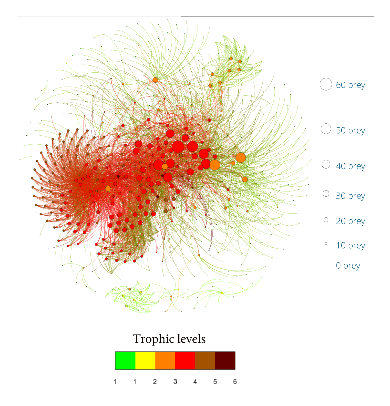
\includegraphics[width=0.5\textwidth]{/home/charles/Talks/Talk_2013Sep23/Antarctic_fweb_review_hires.eps}
\end{figure}
\end{frame}

\begin{frame}{Motivation}
\begin{itemize}
\item Many aspects about the vulnerability of food webs to disturbances in species can be studied by topological and robustness analysis.
\end{itemize}
\begin{figure}
\includegraphics[width=0.5\textwidth]{/home/charles/Talks/Talk_2013Sep23/new_secondary_extinction_preyext.eps}
\end{figure}
\end{frame}



\begin{frame}{Motivation}
\begin{block}<+->{}
However, those approaches don't achieve the consequences of \textbf{individual level disturbances in the stability of ecosystems}. In this direction, we proposed the creation of an \emph{Individual Based Predation and Migration model}.
\end{block} 
\end{frame}

%%%%%%%%%%%%%%%%%%%%%%%%%%%%%%%%%%%%%%%%%%%%%%%%%%%%%%%
\section{\scshape The Model}

\subsection{The Model}

\begin{frame}
\frametitle{The Model}

\includegraphics[width=1.0\textwidth]{/home/charles/Talks/Talk_2013Sep23/matrix.eps}
\end{frame}

\begin{frame}
\centering To study predator-prey and migration dynamics in a landscape.
\begin{figure}
\centering 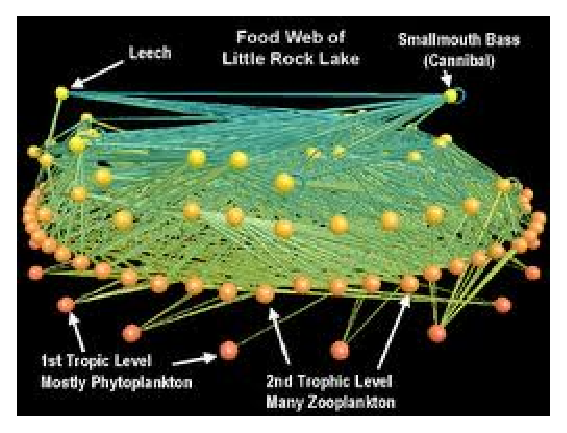
\includegraphics[width=0.4\textwidth]{/home/charles/Talks/Talk_2013Sep23/conectivity_species.eps}
\end{figure}
\end{frame}

\begin{frame}
\centering To study predator-prey and migration dynamics in a landscape.
\begin{figure}
\centering 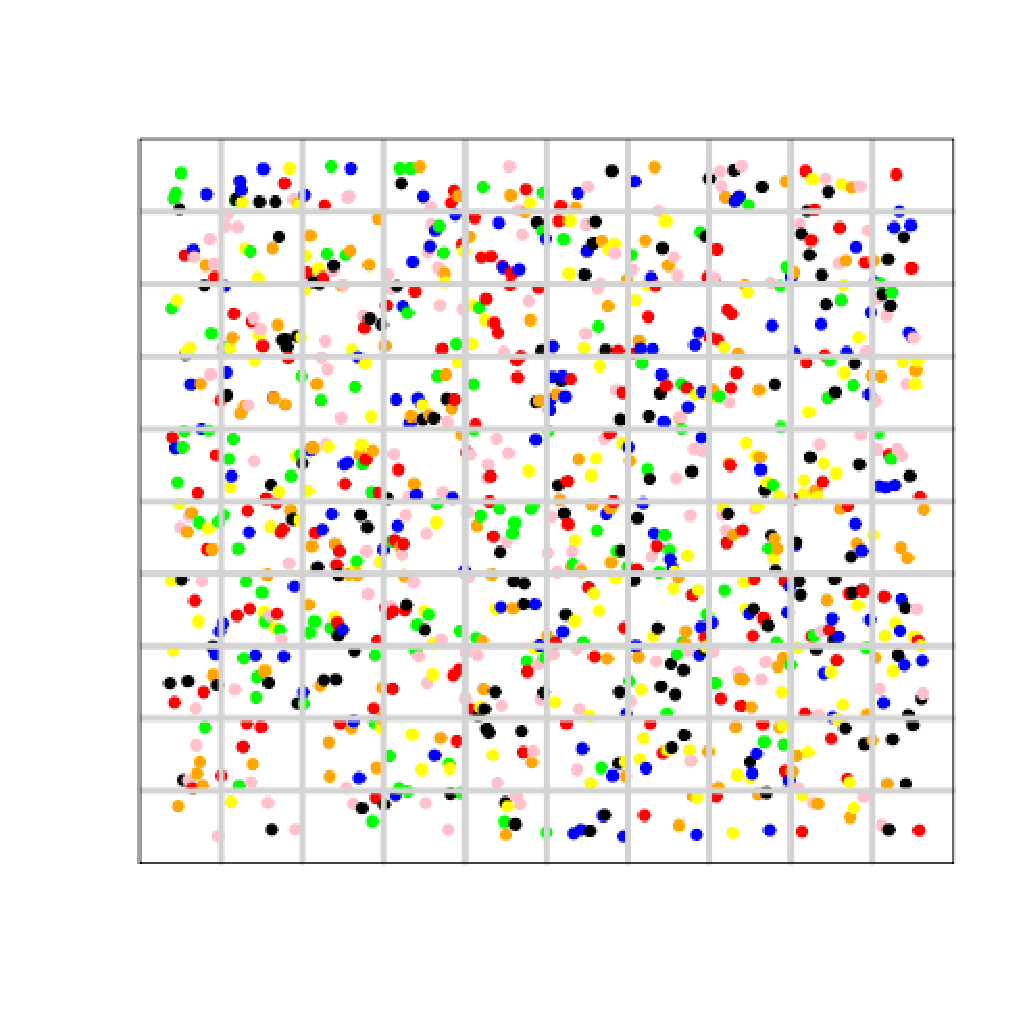
\includegraphics[width=0.7\textwidth]{/home/charles/Talks/Talk_2013Sep23/occuppiedlattice.eps}
\end{figure}
\end{frame}


%%%%%%%%%%%%%
%%%%%%%%%%%%% P R E D A T I O N
%%%%%%%%%%%%%

\subsection{Predation}

\begin{frame}
\frametitle{Predation Dynamics}
\begin{figure}
\includegraphics[width=1.0\textwidth]{/home/charles/Talks/Talk_2013Sep23/FoodWebModel_Predation.eps}
\end{figure}
\end{frame}


\subsection{Migration}

\begin{frame}
\frametitle{Migration Dynamics}
\begin{block}<+->{}
A diffusion dynamic of individuals from its grid cell towards neighbor grid cells based on the \emph{quality of life}: \textbf{differences in the number of predators and preys} in each site. 
\end{block} 
\end{frame}

%%%\begin{frame}
%%%\frametitle{The Equations}
%%%
%%%\tikzstyle{na} = [baseline=-.5ex]
%%%
%%%\begin{itemize}[<+-| alert@+>]
%%%    \item Births (Increasing number of individuals) 
%%%        \tikz \node[coordinate] (n1) {};
%%%\end{itemize}
%%%
%%%\begin{align*}
%%% N^\prime\left(sp\right) & = N\left(sp\right) \times \left\{ \tikz[baseline]{\node[fill=blue!20,anchor=base] (t1) { $\left[ 1 - NDp\left(sp\right) \right]\left[ \sum_{b \in H\left(sp\right)}\rho\left(b\right)Dp\left(b\right) \right]\left[Bp\left(sp\right)\right]$ };}  \right.\nonumber  \\
%%% &\qquad \left. \tikz[baseline]{\node[fill=red!20,anchor=base] (t2) {$- \left[\sum_{c \in P\left(sp\right)}\rho\left(c\right)\left( 1-NDp \left(c \right) \right)\frac{\rho\left(sp\right)}{\sum_{d \in H\left(c\right)}\rho\left(d\right)}Dp\left(sp\right)\right]-\left[NDp\left(sp\right)\right]$ };} \right\} 
%%%\end{align*}
%%%
%%%\begin{itemize}[<+-| alert@+>]
%%%    \item Deaths (Decreasing number of individuals) 
%%%        \tikz \node [coordinate] (n2) {};
%%%\end{itemize}
%%%
%%%% Now it's time to draw some edges between the global nodes. Note that we
%%%% have to apply the 'overlay' style.
%%%\begin{tikzpicture}[overlay]
%%%        \path[->]<1-> (n1) edge [bend left] (t1);
%%%        \path[->]<2-> (n2) edge [bend right] (t2);
%%%\end{tikzpicture}
%%%
%%%\end{frame}
%%%
%%%\begin{frame}
%%%\frametitle{The Parameters}
%%%\begin{block}<+->{}
%%%$\rho(sp)$: Proportion of $sp$. 
%%%\end{block} 
%%%\begin{block}<+->{}
%%%$H(sp)$: Prey Species of $sp$. 
%%%\end{block} 
%%%\begin{block}<+->{}
%%%$P(sp)$: Predator Species of $sp$. 
%%%\end{block} 
%%%\begin{block}<+->{}
%%%\tikz[baseline]{\node[fill=yellow!20,ellipse,anchor=base] (t1) {$Bp(sp)$: Birth Probability of $sp$.};} 
%%%\end{block} 
%%%\begin{block}<+->{}
%%%\tikz[baseline]{\node[fill=yellow!20,ellipse,anchor=base] (t1) {$Dp(sp)$: Death Probability of $sp$.};} 
%%%\end{block} 
%%%\begin{block}<+->{}
%%%\tikz[baseline]{\node[fill=yellow!20,ellipse,anchor=base] (t1) {$NDp(sp)$: Natural Death Probability of $sp$.};} 
%%%\end{block} 
%%%\end{frame}
%%%
%%%%%%%%%%%%%%%%%%
%%%%%%%%%%%%%%%%%%% B I R T H      P R O B A B I L I T Y
%%%%%%%%%%%%%%%%%%
%%%
%%%\begin{frame}
%%%\frametitle{Self-Organized Parameters}
%%%\centering 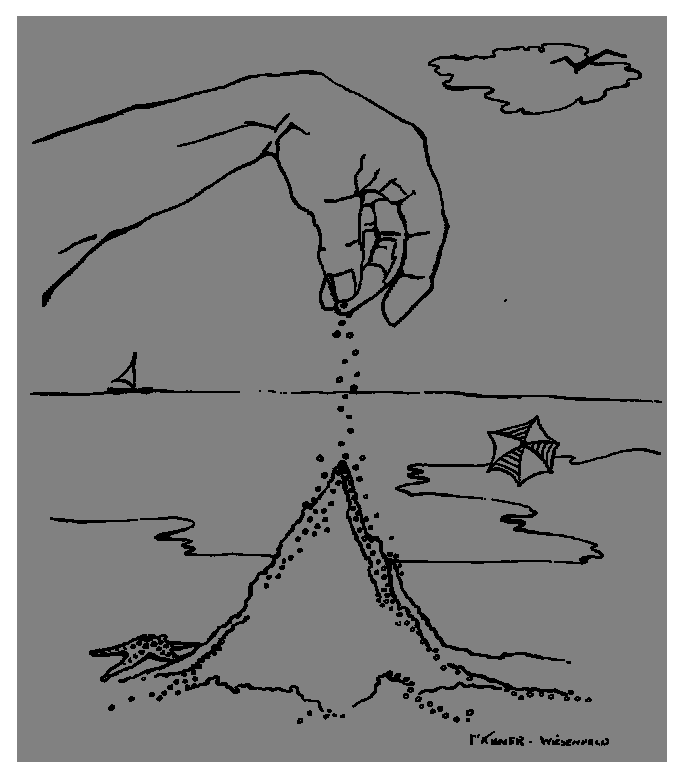
\includegraphics[width=0.5\textwidth]{/home/charles/Talks/Talk_2013Sep23/SOC.eps}
%%%\end{frame}
%%%
%%%\begin{frame}
%%%\frametitle{Self-Organized Parameters: Birth}
%%%\tikzstyle{na} = [baseline=-.5ex]
%%%\begin{itemize}[<+-| alert@+>]
%%%    \item Availability of Space
%%%        \tikz \node[coordinate] (n1) {};
%%%\end{itemize}
%%%% Below we mix an ordinary equation with TikZ nodes. Note that we have to
%%%% adjust the baseline of the nodes to get proper alignment with the rest of
%%%% the equation.
%%%
%%%\begin{align*}
%%%Bp\left(sp\right) & = \tikz[baseline]{\node[fill=blue!20,ellipse,anchor=base] (t1) {$\left[1 - \rho\left(sp\right)\right]$};} \times \tikz[baseline]{\node[fill=red!20,anchor=base] (t2) {$\left[\sum_{b \in H\left(sp\right)}\rho\left(b\right)\left(1-\sum_{c \in P\left(b\right)}\rho\left(c\right)\right)\right]$};} \\
%%%& \times \tikz[baseline]{\node[fill=green!20,anchor=base] (t3) {$\left[1-\sum_{c \in P\left(sp\right)}\rho\left(c\right) \right]$};}
%%%\end{align*}
%%%
%%%\begin{itemize}[<+-| alert@+>]
%%%    \item Safety 
%%%        \tikz\node [coordinate] (n3) {};
%%%    \item Availability of Resources 
%%%        \tikz\node [coordinate] (n2) {};
%%%\end{itemize}
%%%% Now it's time to draw some edges between the global nodes. Note that we
%%%% have to apply the 'overlay' style.
%%%\begin{tikzpicture}[overlay]
%%%        \path[->]<1-> (n1) edge [bend left] (t1);
%%%        \path[->]<2-> (n3) edge [out=0, in=-90] (t3);
%%%        \path[->]<3-> (n2) edge [bend right] (t2);
%%%\end{tikzpicture}
%%%\end{frame}
%%%
%%%%%%%%%%%%%
%%%%%%%%%%%% O B S E R V A T I O N S
%%%%%%%%%%%%%
%%%
%%%\begin{frame}
%%%\frametitle{Observations}
%%%\begin{block}<+->{}
%%%\textbf{Availability of Resources} of \textbf{Basal Species} is 1.0
%%%\end{block} 
%%%\end{frame}
%%%
%%%%%%%%%%%%%%%%%%%%%%%%%%
%%%%%%%%%%%%%%%%%%%%%%%%%%% D E A T H     P R O B A B I L I T Y
%%%%%%%%%%%%%%%%%%%%%%%%%%
%%%
%%%
%%%\begin{frame}
%%%\frametitle{Self-Organized Parameters: Death}
%%%
%%%\tikzstyle{na} = [baseline=-.5ex]
%%%\begin{itemize}[<+-| alert@+>]
%%%    \item Intraespecific Competition
%%%        \tikz \node[coordinate] (n1) {};
%%%\end{itemize}
%%%% Below we mix an ordinary equation with TikZ nodes. Note that we have to
%%%% adjust the baseline of the nodes to get proper alignment with the rest of
%%%% the equation.
%%%
%%%\begin{align*}
%%%Dp\left(sp\right) & = \tikz[baseline]{\node[fill=blue!20,ellipse,anchor=base] (t1) {$\left[\rho\left(sp\right)\right]$};} \times \tikz[baseline]{\node[fill=red!20,anchor=base] (t2) {$\left[\sum_{b \in H\left(sp\right)}\left(1-\rho\left(b\right)\right)\left(\sum_{c \in P\left(b\right)}\rho\left(c\right)\right)\right]$};} \\ 
%%%& \times \tikz[baseline]{\node[fill=green!20,anchor=base] (t3) {$\left[1-\sum_{c \in P\left(sp\right)}\rho\left(c\right) \right]$};} 
%%%\end{align*}
%%%
%%%\begin{itemize}[<+-| alert@+>]
%%%    \item Surprise effect 
%%%        \tikz\node [coordinate] (n3) {};
%%%    \item Privation of Resources
%%%        \tikz\node [coordinate] (n2) {};
%%%\end{itemize}
%%%% Now it's time to draw some edges between the global nodes. Note that we
%%%% have to apply the 'overlay' style.
%%%\begin{tikzpicture}[overlay]
%%%        \path[->]<1-> (n1) edge [bend left] (t1);
%%%        \path[->]<2-> (n3) edge [out=0, in=-90] (t3);
%%%        \path[->]<3-> (n2) edge [bend right] (t2);
%%%\end{tikzpicture}
%%%
%%%\end{frame}
%%%
%%%%%%%%%%%%%
%%%%%%%%%%%% O B S E R V A T I O N S
%%%%%%%%%%%%%
%%%
%%%\begin{frame}
%%%\frametitle{Observations}
%%%\begin{block}<+->{}
%%%\textbf{Death Probability} of \textbf{Basal Species} is 1.0
%%%\end{block} 
%%%\end{frame}
%%%
%%%%%%%%%%%%%%%%%%%%%%%%%%
%%%%%%%%%%%%%%%%%%%%%%%%%%% N A T U R A L     D E A T H     P R O B A B I L I T Y
%%%%%%%%%%%%%%%%%%%%%%%%%%
%%%
%%%\begin{frame}
%%%\frametitle{Self-Organized Parameters: Natural Death}
%%%
%%%\tikzstyle{na} = [baseline=-.5ex]
%%%\begin{itemize}[<+-| alert@+>]
%%%    \item Intraespecific Competition
%%%        \tikz \node[coordinate] (n1) {};
%%%\end{itemize}
%%%% Below we mix an ordinary equation with TikZ nodes. Note that we have to
%%%% adjust the baseline of the nodes to get proper alignment with the rest of
%%%% the equation.
%%%
%%%\begin{align*}
%%%NDp\left(sp\right) & = \tikz[baseline]{\node[fill=blue!20,ellipse,anchor=base] (t1) {$\left[\rho\left(sp\right)\right]$};} \times \tikz[baseline]{\node[fill=red!20,anchor=base] (t2) {$\left[\sum_{b \in H\left(sp\right)}\left(1-\rho\left(b\right)\right)\left(\sum_{c \in P\left(b\right)}\rho\left(c\right)\right)\right]$};} \\ 
%%%& \times \tikz[baseline]{\node[fill=green!20,anchor=base] (t3) {$\left[1-\sum_{c \in P\left(sp\right)}\rho\left(c\right) \right]$};} 
%%%\end{align*}
%%%
%%%\begin{itemize}[<+-| alert@+>]
%%%    \item Absence of predators 
%%%        \tikz\node [coordinate] (n3) {};
%%%    \item Privation of Resources
%%%        \tikz\node [coordinate] (n2) {};
%%%\end{itemize}
%%%% Now it's time to draw some edges between the global nodes. Note that we
%%%% have to apply the 'overlay' style.
%%%\begin{tikzpicture}[overlay]
%%%        \path[->]<1-> (n1) edge [bend left] (t1);
%%%        \path[->]<2-> (n3) edge [out=0, in=-90] (t3);
%%%        \path[->]<3-> (n2) edge [bend right] (t2);
%%%\end{tikzpicture}
%%%
%%%\end{frame}
%%%
%%%
%%%%%%%%%%%%%%%%
%%%%%%%%%%%%%%%% S P E C I E S     C A R R Y I N G     C A P A C I T Y
%%%%%%%%%%%%%%%%
%%%
%%%
%%%\begin{frame}
%%%\frametitle{Self-Organized Parameters: Carrying Capacity (for each species in each site)}
%%%
%%%\tikzstyle{na} = [baseline=-.5ex]
%%%
%%%\begin{itemize}[<+-| alert@+>]
%%%    \item Availability of Resources 
%%%        \tikz \node[coordinate] (n1) {};
%%%\end{itemize}
%%%% Below we mix an ordinary equation with TikZ nodes. Note that we have to
%%%% adjust the baseline of the nodes to get proper alignment with the rest of
%%%% the equation.
%%%%a*d_prey/d_predOfprey
%%%\begin{align*}
%%%CC\left(sp\right) & =  \tikz[baseline]{\node[fill=red!20,ellipse,anchor=base] (t2) {$\left[\sum_{b \in H\left(sp\right)}\frac{\left(\rho\left(b\right)\right)}{\left(\sum_{c \in P\left(b\right)}\rho\left(c\right)\right)}\right]$};}
%%%\end{align*}
%%%
%%%% Now it's time to draw some edges between the global nodes. Note that we
%%%% have to apply the 'overlay' style.
%%%\begin{tikzpicture}[overlay]
%%%        \path[->]<1-> (n1) edge [bend left] (t1);
%%%\end{tikzpicture}
%%%
%%%\end{frame}

%%%%%%%%%%%%%%%%
%%%%%%%%%%%%%%%% M O B I L I T Y 
%%%%%%%%%%%%%%%% 
 
%%%%%%\subsection{Mobility}
%%%%%%
%%%%%%\begin{frame}
%%%%%%\frametitle{Mobility Dynamics}
%%%%%%%\includegraphics[width=1.0\textwidth]{/home/charles/Talks/Talk_2013Sep23/mobility.eps}
%%%%%%\end{frame}
%%%%%%
%%%%%%\begin{frame}
%%%%%%\frametitle{Mobility Dynamics}
%%%%%%
%%%%%%\tikzstyle{na} = [baseline=-.5ex]
%%%%%%
%%%%%%\begin{itemize}[<2->]
%%%%%%    \item Number of individuals of species \emph{sp} at site \emph{i} 
%%%%%%        \tikz \node[coordinate] (n1) {};
%%%%%%\end{itemize}
%%%%%%
%%%%%%\vspace{2cm}
%%%%%%
%%%%%%$\Delta N_{sp}\left(i\right) = \sum_{j \in Neigh\left(i\right)} \left( \left( N_{sp}(j) \; M_{sp}(j,i) \; - \; \tikz[baseline]{\node[fill=blue!20,anchor=base] (t1) {$N_{sp}(i) $};} \tikz[baseline]{\node[fill=red!20,anchor=base] (t2) {$M_{sp}(i,j)$};} \right) \right)$
%%%%%%
%%%%%%\vspace{2cm}
%%%%%%
%%%%%%\begin{itemize}[<3->]
%%%%%%    \item Mobility of species \emph{sp} from site \emph{i} to \emph{j} 
%%%%%%        \tikz\node [coordinate] (n2) {};
%%%%%%\end{itemize}
%%%%%%% Now it's time to draw some edges between the global nodes. Note that we
%%%%%%% have to apply the 'overlay' style.
%%%%%%\begin{tikzpicture}[overlay]
%%%%%%        \path[->]<2-> (n1) edge [bend left] (t1);
%%%%%%        \path[->]<3-> (n2) edge [bend right] (t2);
%%%%%%\end{tikzpicture}
%%%%%%
%%%%%%\end{frame}
%%%%%%
%%%%%%\begin{frame}
%%%%%%\frametitle{Mobility of species \emph{sp}}
%%%%%%\small{$M(i,j) = \overbrace{ \left[ \lambda^{i} \frac{ \Delta_{ij}\,f\,\Theta \left(\Delta_{ij}\,f\,\right) }{ \sum_{k \in Neigh\left(i\right)}\Delta_{ik}\,f\,\Theta \left(\Delta_{ik}\,f\,\right) }\right]}^{Biotic} \overbrace{\left[w_{ij} \frac{ \Delta_{ij}\,f_{\eta}\,\Theta \left(\Delta_{ij}\,f_{\eta}\,\right) }{ \sum_{k \in Neigh\left(i\right)}\Delta_{ik}\,f_{\eta}\,\Theta \left(\Delta_{ik}\,f_{\eta}\,\right) }\right]}^{Abiotic}$}
%%%%%%\vspace{0.5cm}
%%%%%%\pause
%%%%%%$$
%%%%%%\Delta_{ij}\,f = f^{i,j} - f^{j,i}\left\{ \begin{array}{rl}
%%%%%% f^{i,j} = \rho_{H}(j) + \rho_{P}(i) \\
%%%%%% f^{j,i} = \rho_{H}(i) + \rho_{P}(j) \\
%%%%%%       \end{array} \right.
%%%%%%$$
%%%%%%\pause
%%%%%%\vspace{0.5cm}
%%%%%%\centering $\lambda^{i} = \frac{1}{2} \left( 1 - RE^{i} \right)$ \\
%%%%%%\vspace{0.25cm}
%%%%%%\centering $ RE^{i} = \frac{ New^{t} }{ N^{t} }$
%%%%%%
%%%%%%\end{frame}
%%%%%%
%%%%%%
%%%%%%\begin{frame}
%%%%%%\frametitle{Mobility}
%%%%%%\small{$M(i,j) = \overbrace{ \left[ \lambda(i) \frac{ \Delta_{ij}\,f\,\Theta \left(\Delta_{ij}\,f\,\right) }{ \sum_{k \in Neigh\left(i\right)}\Delta_{ik}\,f\,\Theta \left(\Delta_{ik}\,f\,\right) }\right]}^{Biotic} \overbrace{\left[w_{ij} \left( 1 - \frac{ \Delta_{ij}\,f_{\eta}\,\Theta \left(\Delta_{ij}\,f_{\eta}\,\right) }{ \sum_{k \in Neigh\left(i\right)}\Delta_{ik}\,f_{\eta}\,\Theta \left(\Delta_{ik}\,f_{\eta}\,\right) }\right)\right]}^{Abiotic}$}
%%%%%%\vspace{0.5cm}
%%%%%%\pause
%%%%%%$$
%%%%%% \Delta_{ij}\,f_{\eta} = f_{\eta}^{j} - f_{\eta}^{i} \left\{ \begin{array}{rl}
%%%%%% f_{\eta}^{i} = \eta_{sp}^{*} - \eta_{sp}^{i} \\
%%%%%% f_{\eta}^{j} = \eta_{sp}^{*} - \eta_{sp}^{i} \\
%%%%%%       \end{array} \right.
%%%%%%$$
%%%%%%\vspace{0.5cm}
%%%%%%\pause
%%%%%%$$
%%%%%% \left\{ \begin{array}{rl}
%%%%%% w_{ij} = Connectivity \; between \; sites  \; i  \; and  \; j\\
%%%%%%\end{array} \right.
%%%%%%$$
%%%%%%\end{frame}
%%%%%%
%%%%%%%%%%%%%%%%%%%%%% 
%%%%%%%%%%%%%%%%%%%%%%

\section{\scshape Simulations}

\begin{frame}
\frametitle{Results}
\centering \includegraphics[width=0.75\textwidth]{/home/charles/Talks/Talk_2013Sep23/result.eps}
\end{frame}

\begin{frame}
\centering We populate each grid cells of the landscape with a random number of individuals of different species. The trophic relationships among the species are defined by a food web.
\begin{figure}
\centering 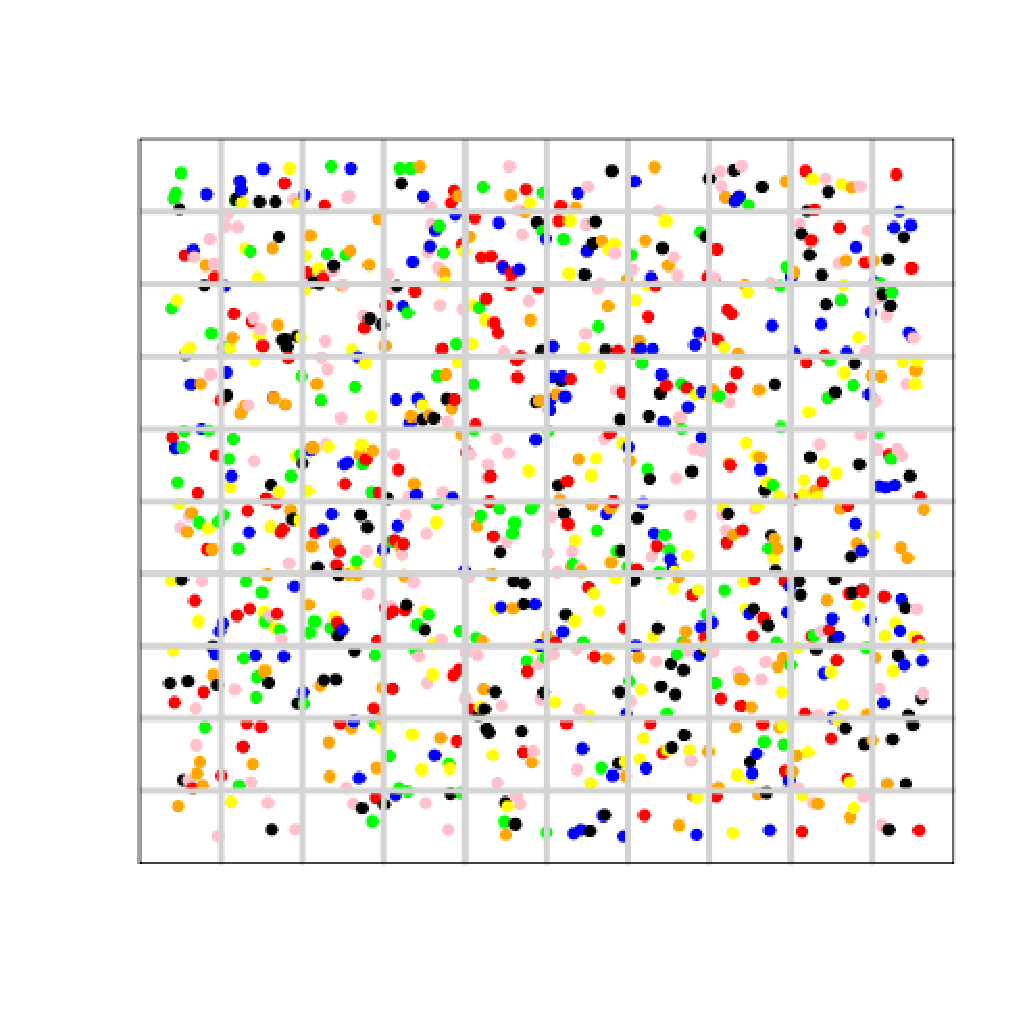
\includegraphics[width=0.7\textwidth]{/home/charles/Talks/Talk_2013Sep23/occuppiedlattice.eps}
\end{figure}
\end{frame}

\subsection{Steady State}

%%%%%%%%%%%%% 9      S P E C I E S 

\begin{frame}
\frametitle{9 species food web}
\begin{figure}
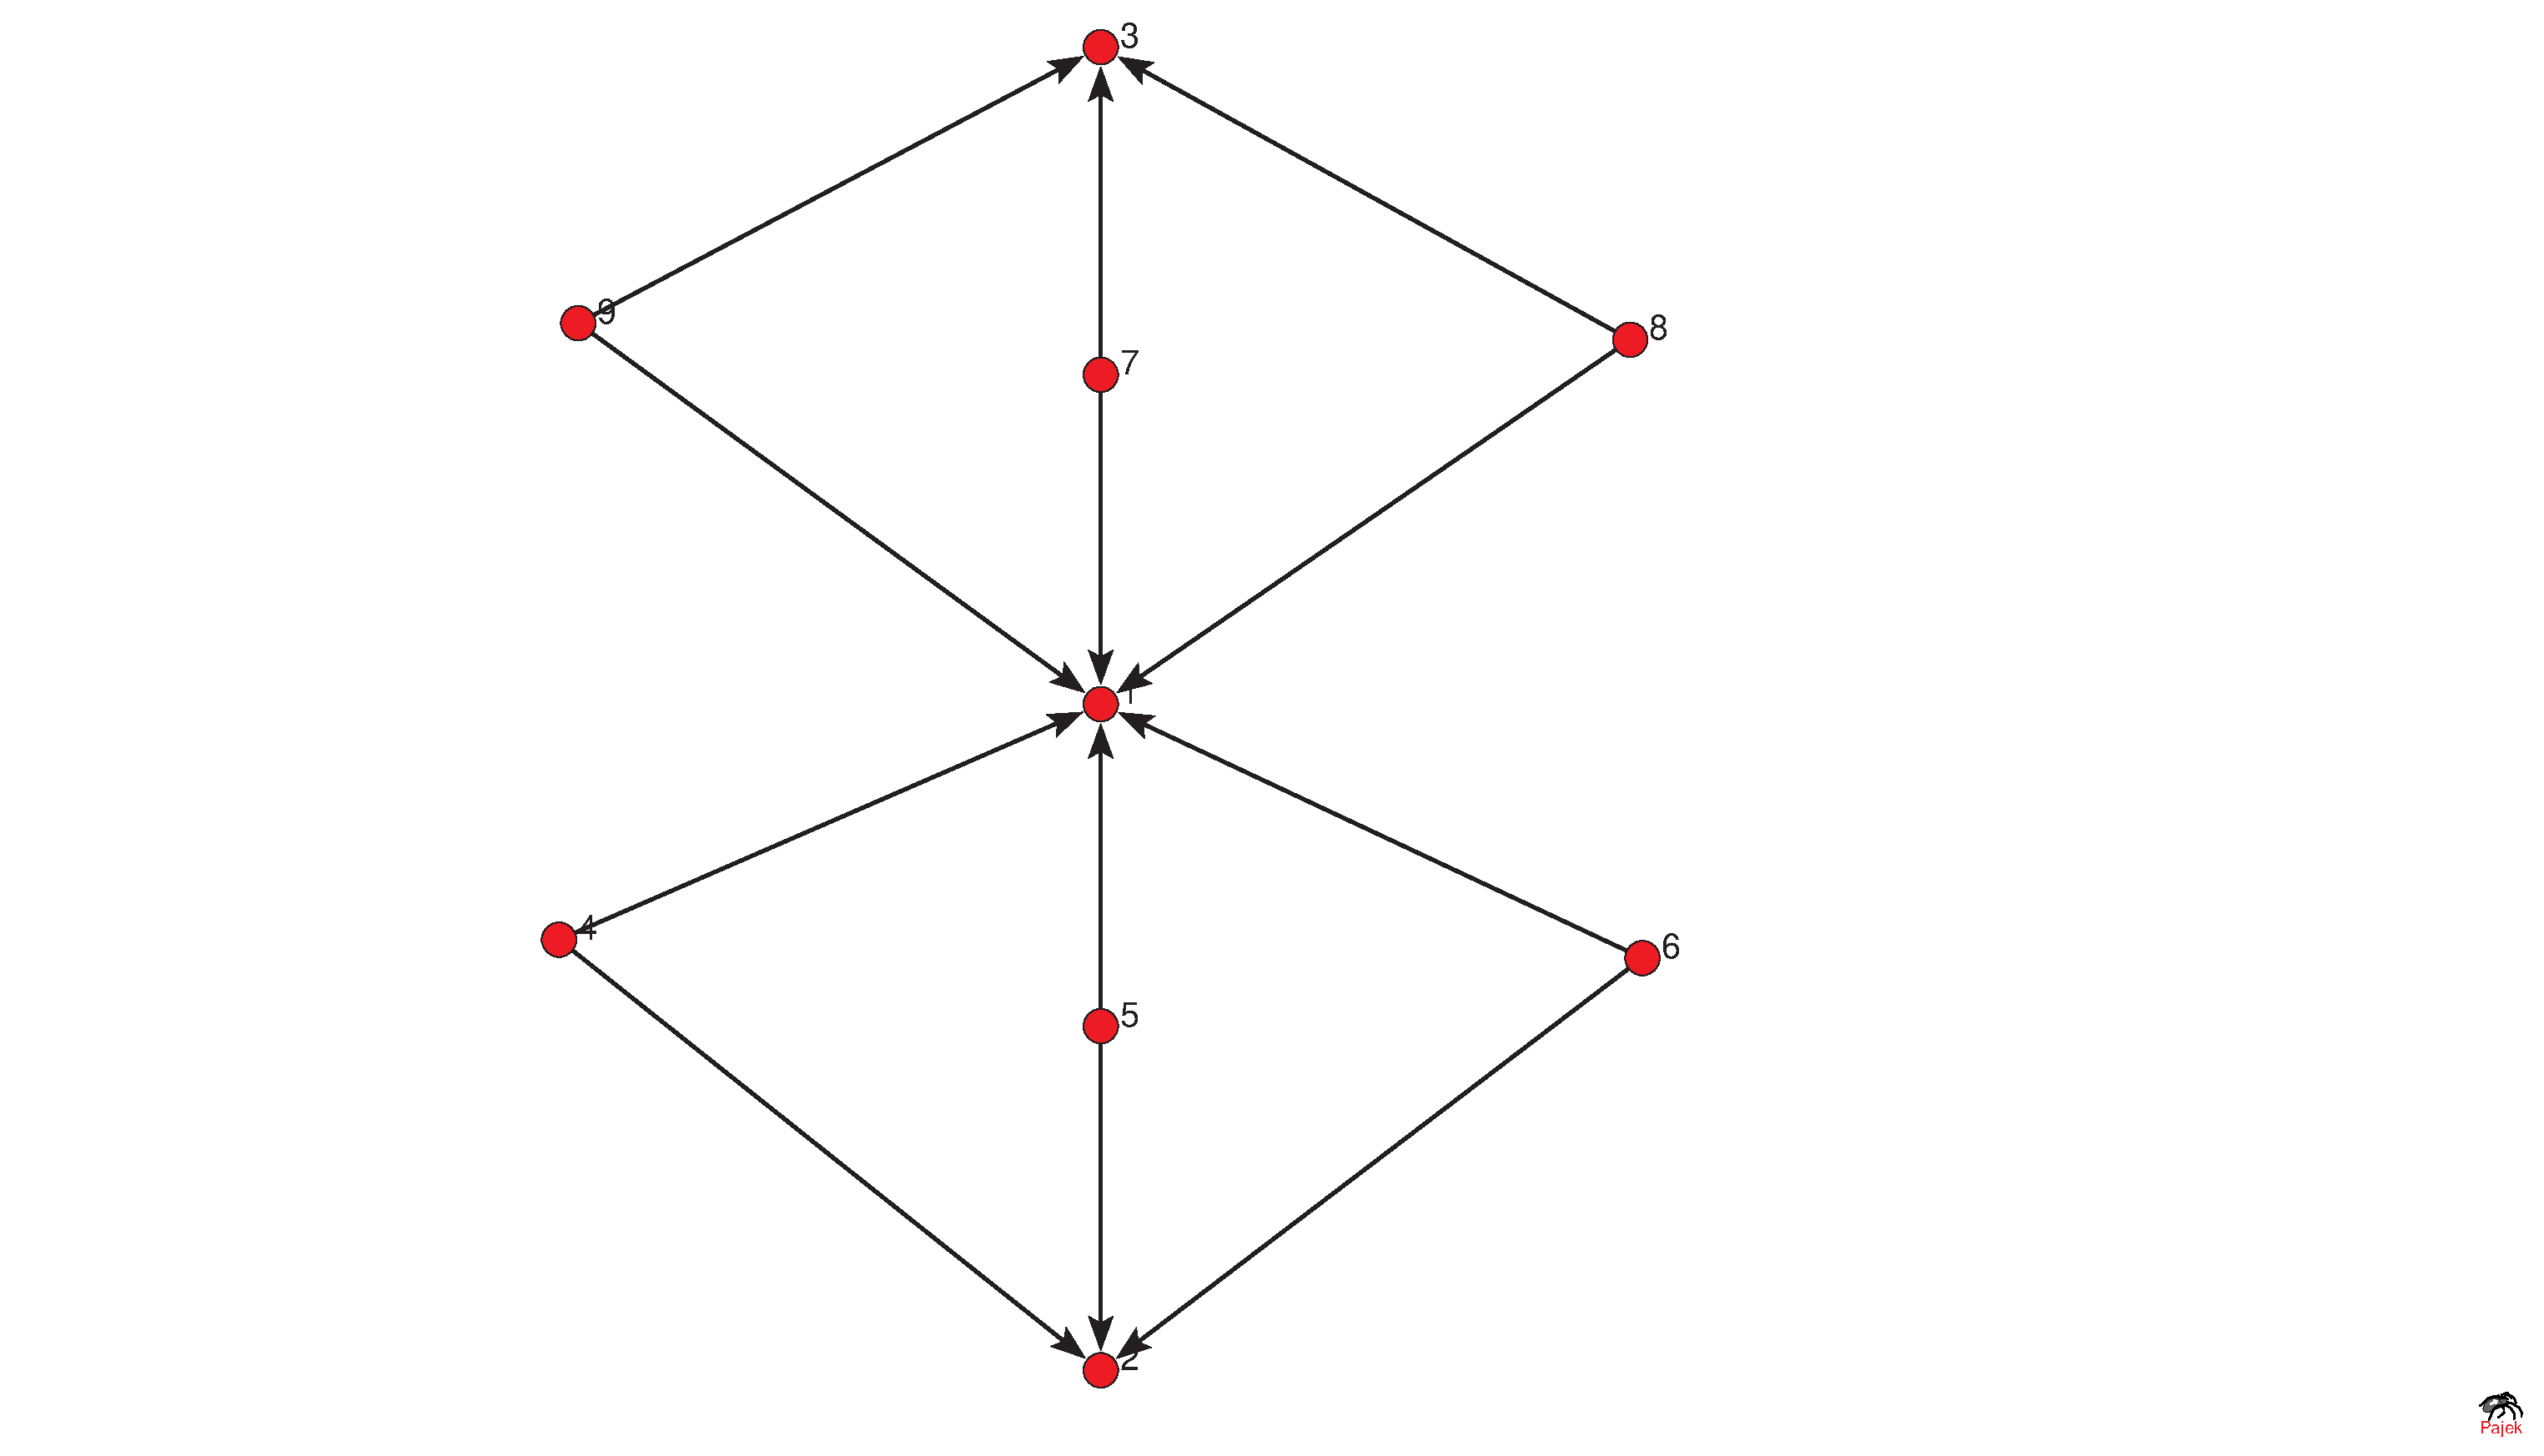
\includegraphics[width=1.0\textwidth]{/home/charles/Talks/Talk_2013Sep23/FoodWeb_9species.eps}
\end{figure}
\end{frame}

%\begin{frame}
%\frametitle{Maximum Start = 10000 Inds.}
%\begin{figure}
%\includegraphics[angle=270,width=0.8\textwidth]{/home/charles/Talks/Talk_2013Sep23/AverIndInTime_9species_30Real_10000.eps}
%\end{figure}
%\end{frame}

\begin{frame}
\frametitle{Maximum Start = 100 and 1000 Inds.}
\begin{figure}
\includegraphics[angle=270,width=0.8\textwidth]{/home/charles/Talks/Talk_2013Sep23/AverIndInTime_30Real_100_1000.eps}
\end{figure}
\end{frame}

%%%%%%%%%%%% 3 0   S P E C I E S

\begin{frame}
\frametitle{30 species food web}
\begin{figure}
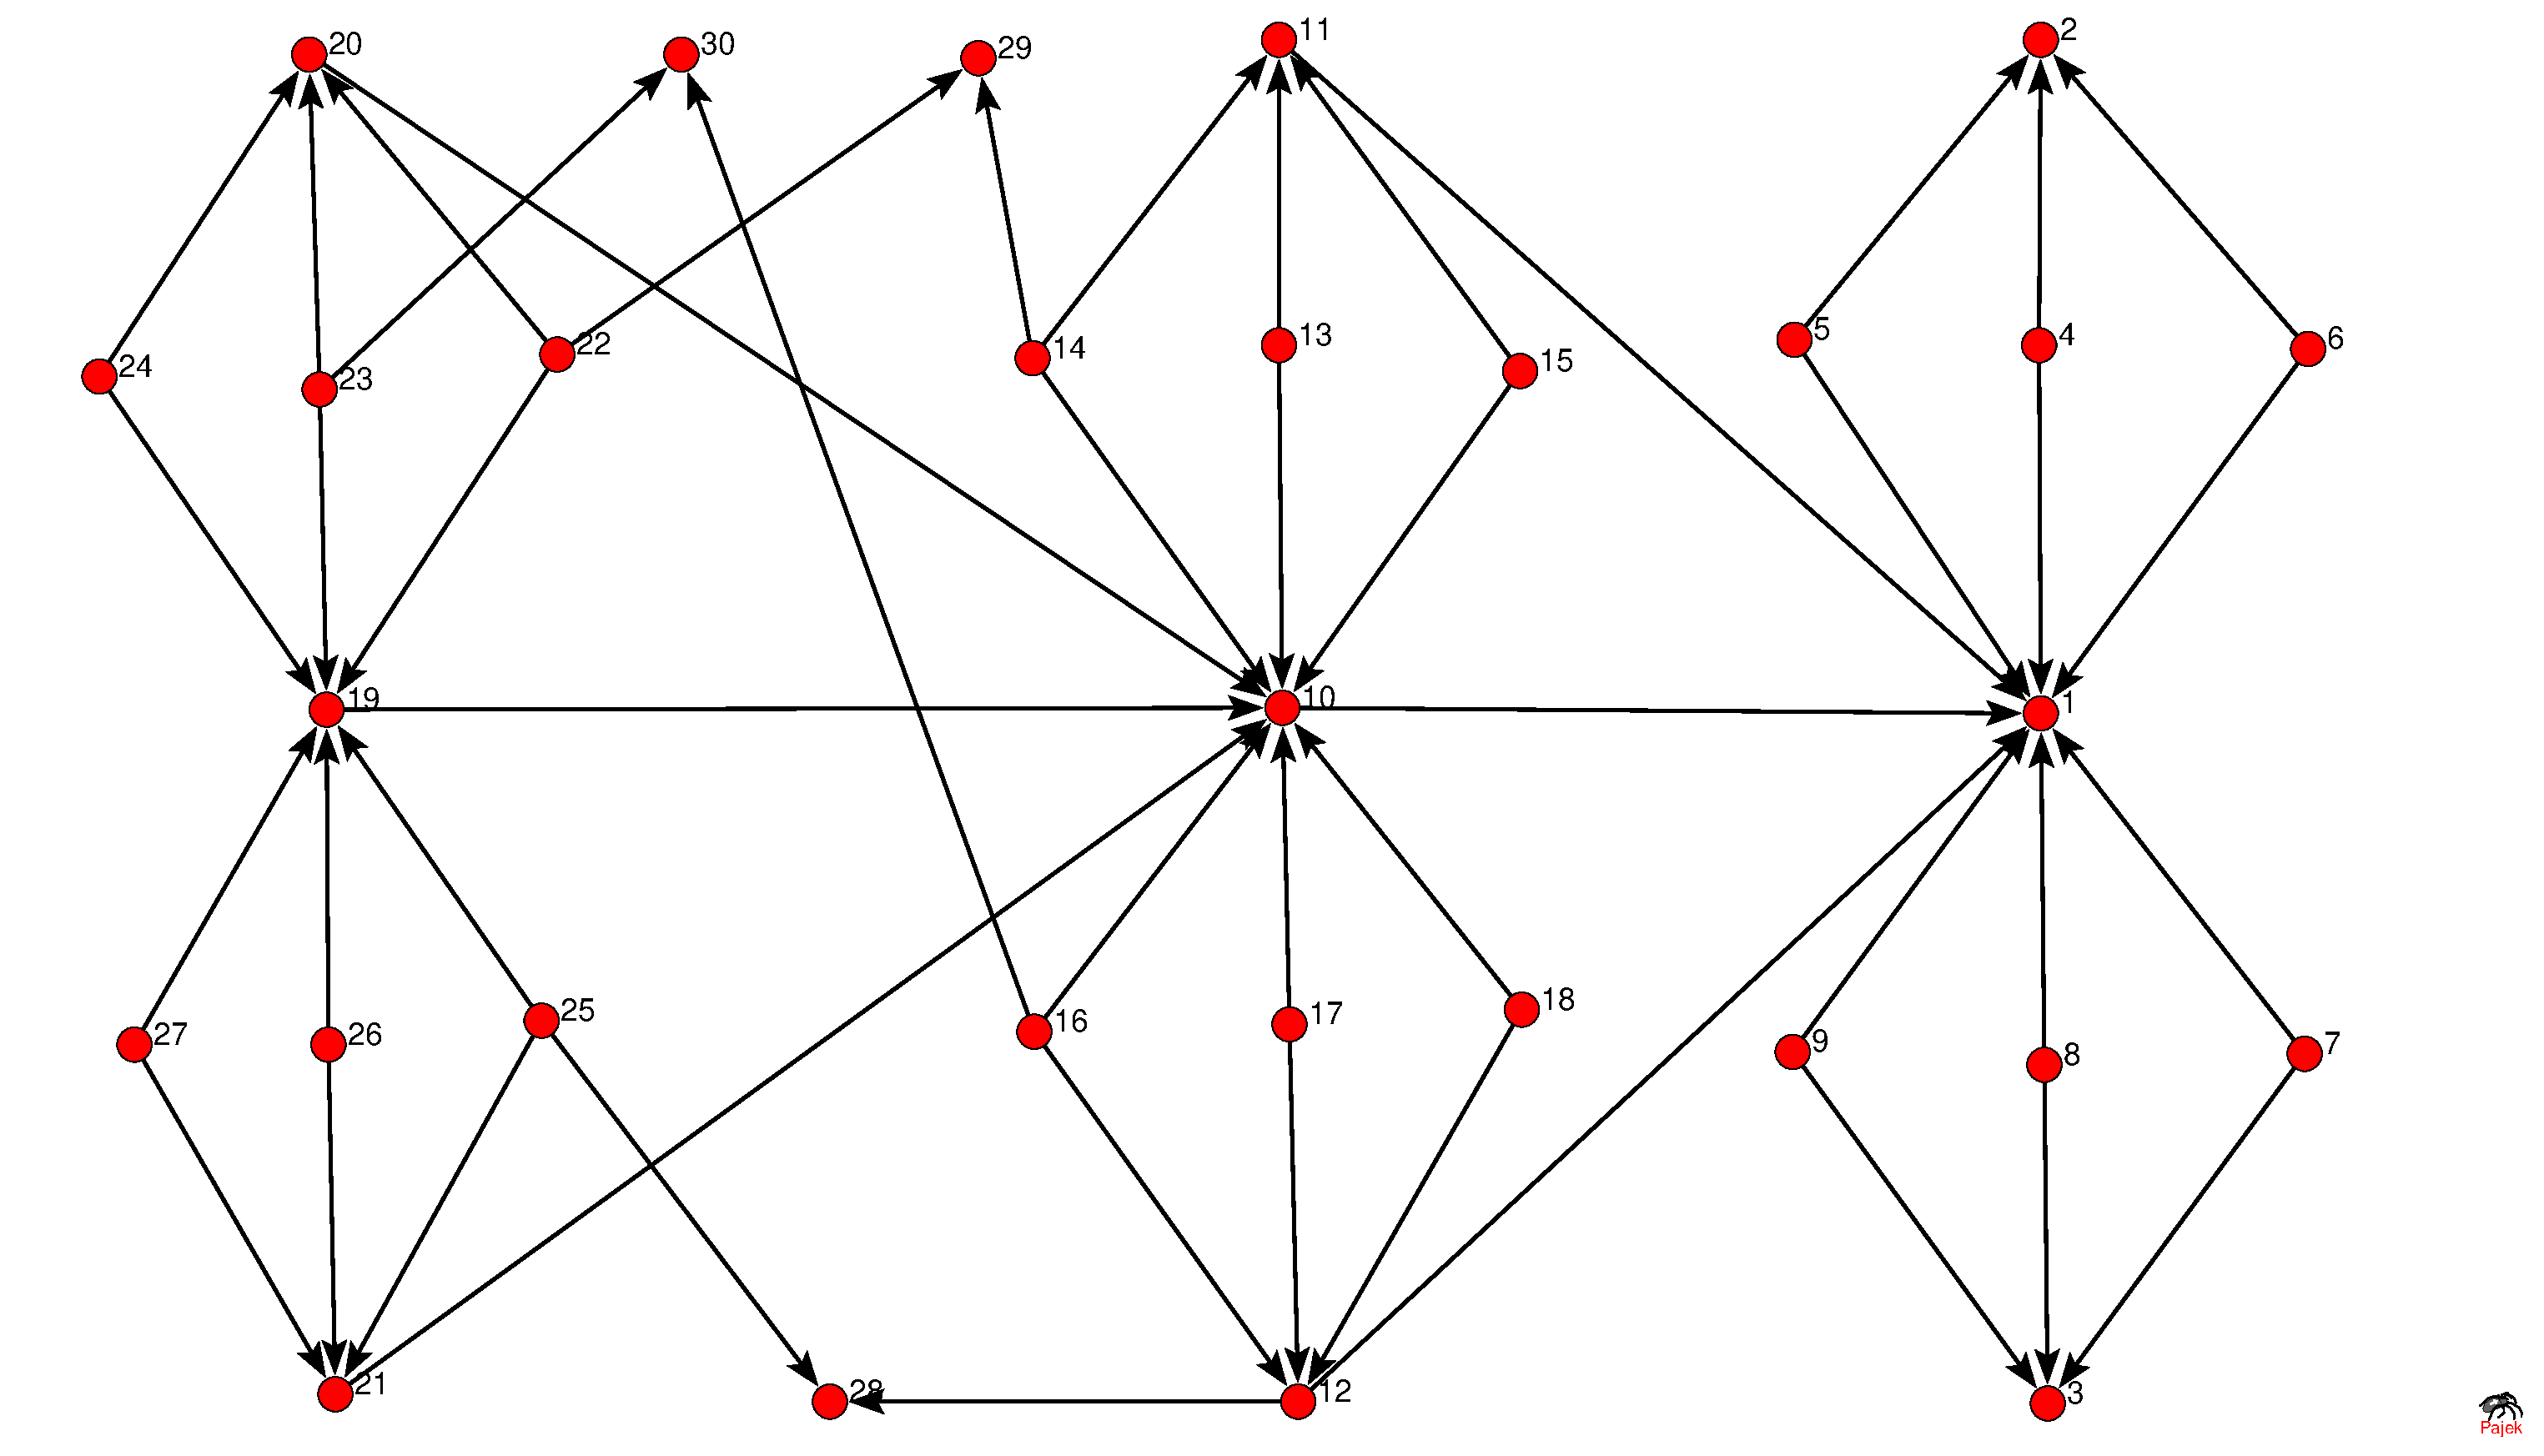
\includegraphics[width=1.0\textwidth]{/home/charles/Talks/Talk_2013Sep23/FoodWeb_30bloques9.eps}
\end{figure}
\end{frame}

\begin{frame}
\frametitle{Maximum Start = 10 Inds.}
\begin{figure}
\includegraphics[angle=270,width=0.8\textwidth]{/home/charles/Talks/Talk_2013Sep23/AverIndInTime_50Real_10Ind.eps}
\end{figure}
\end{frame}

%%\begin{frame}
%%\frametitle{Individuals in Time: Maximum Start = 10}
%%\begin{figure}
%%\framezoom<1><1>[border](0.5cm,6.0cm)(1cm,1cm)
%%\framezoom<1><2>[border](5.5cm,3.0cm)(1cm,1cm)
%%\framezoom<1><3>[border](5.5cm,4.0cm)(1cm,1cm)
%%\framezoom<1><4>[border](5.5cm,5.0cm)(1cm,1cm)
%%\framezoom<1><5>[border](5.5cm,6.0cm)(1cm,1cm)
%%\includegraphics[angle=270,width=0.9\textwidth]{/home/charles/Talks/Talk_2013Sep23/AverIndInTime_50Real_10Ind.eps}
%%\end{figure}
%%\end{frame}

\begin{frame}
\frametitle{Maximum Start = 1000 Inds.}
\begin{figure}
\includegraphics[angle=270,width=0.8\textwidth]{/home/charles/Talks/Talk_2013Sep23/AverIndInTime_50Real_1000Ind.eps}
\end{figure}
\end{frame}

%%\begin{frame}
%%\frametitle{Individuals in Time: Maximum Start = 1000}
%%\begin{figure}
%%\framezoom<1><1>[border](1.5cm,4.0cm)(1cm,1cm)
%%\framezoom<1><2>[border](2.5cm,3.0cm)(1cm,1cm)
%%\framezoom<1><3>[border](2.5cm,4.0cm)(1cm,1cm)
%%\framezoom<1><4>[border](2.5cm,5.0cm)(1cm,1cm)
%%\framezoom<1><5>[border](4.5cm,3.0cm)(1cm,1cm)
%%\framezoom<1><6>[border](4.5cm,4.0cm)(1cm,1cm)
%%\framezoom<1><7>[border](4.5cm,5.0cm)(1cm,1cm)
%%\includegraphics[angle=270,width=0.8\textwidth]{/home/charles/Talks/Talk_2013Sep23/AverIndInTime_50Real_1000Ind.eps}
%%\end{figure}
%%\end{frame}
%
%
%%%%%%%%%%%%%% 7 5      S P E C I E S 

\begin{frame}
\frametitle{75 species food web}
\begin{figure}
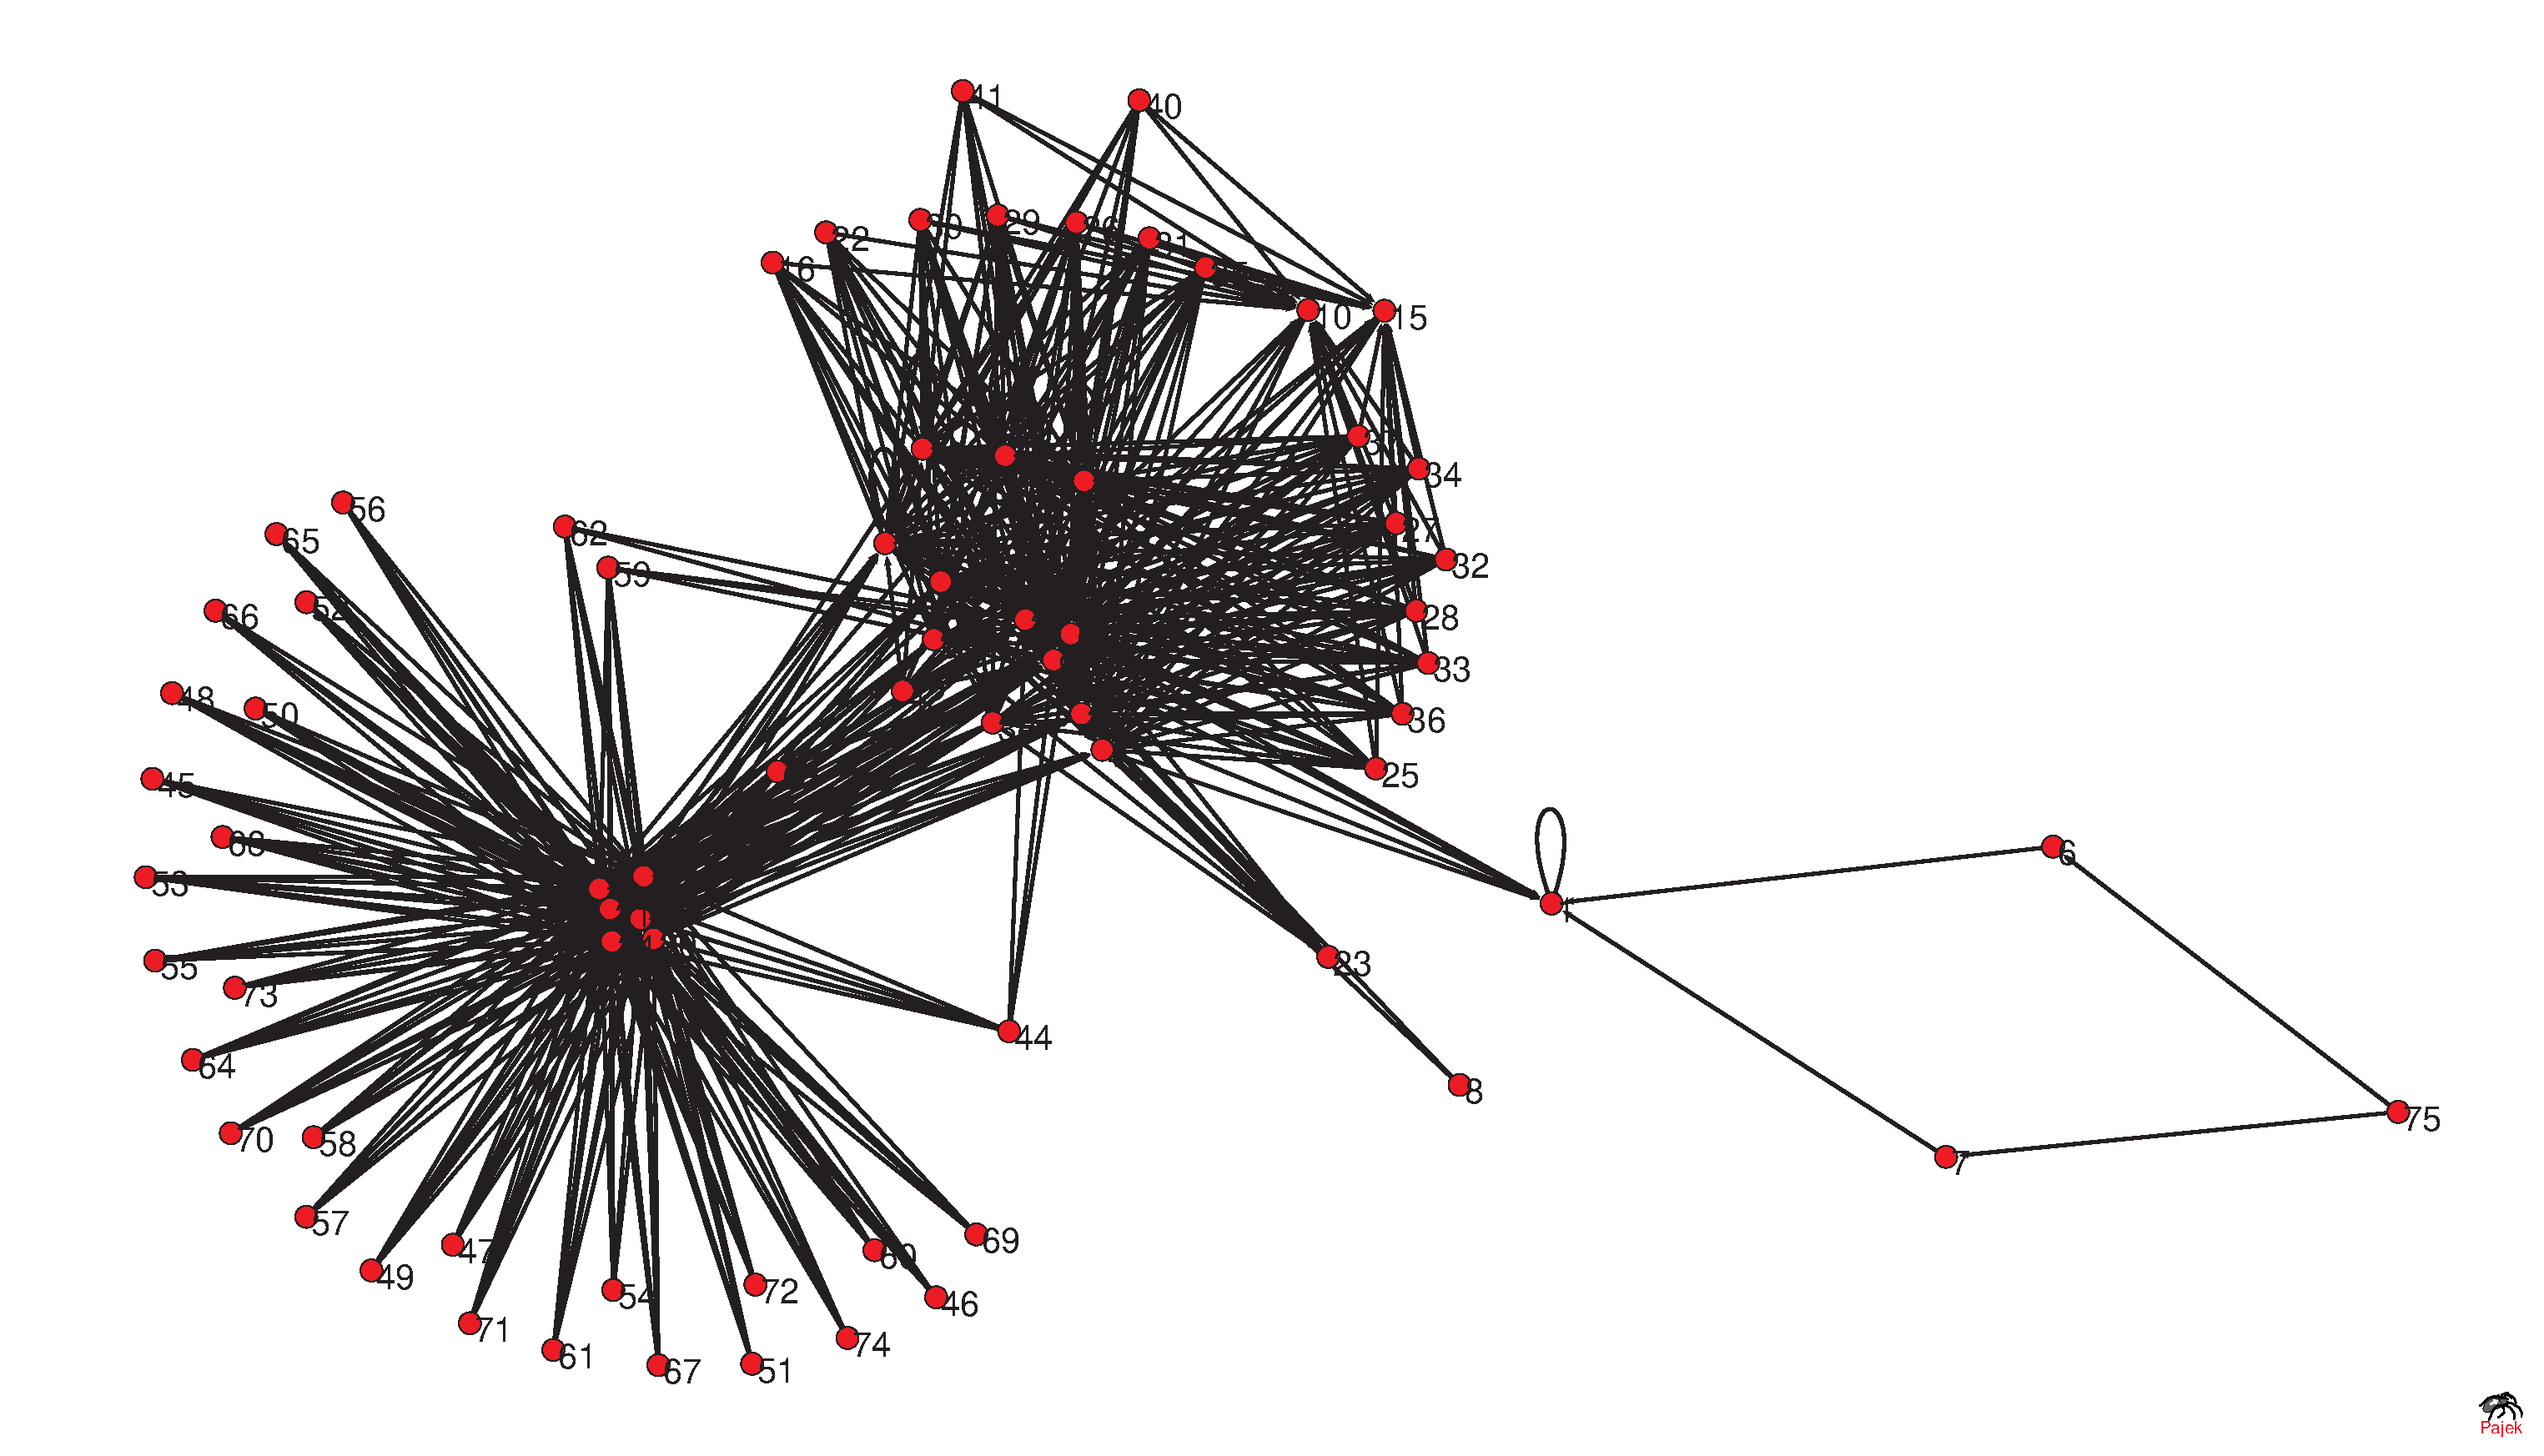
\includegraphics[width=1.0\textwidth]{/home/charles/Talks/Talk_2013Sep23/FoodWeb_75species_Dunne}
\end{figure}
\end{frame}

\begin{frame}
\frametitle{Maximum Start = 100 Inds.}
\begin{figure}
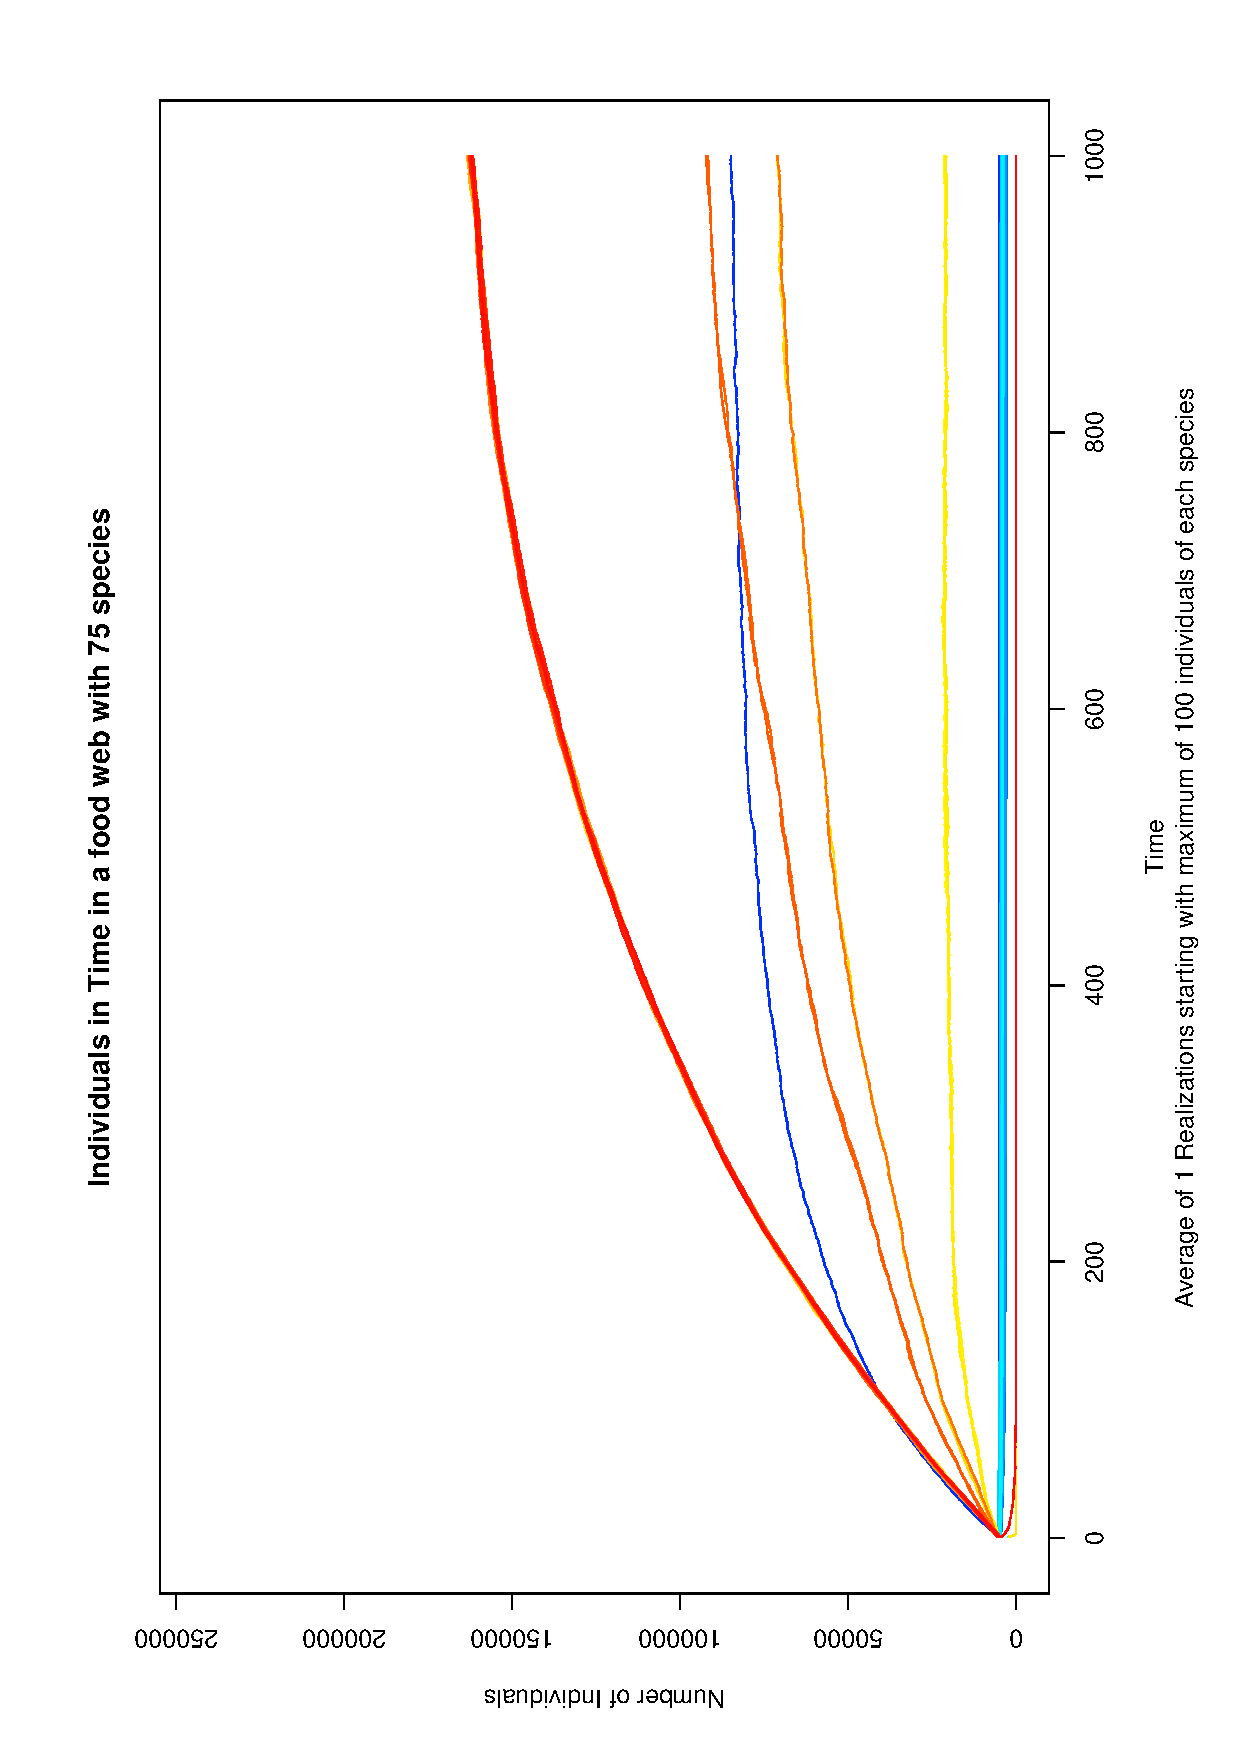
\includegraphics[angle=270,width=0.8\textwidth]{/home/charles/Talks/Talk_2013Sep23/AverIndInTime_75Dunne_1000}
\end{figure}
\end{frame}

\begin{frame}
\frametitle{Stability of the Food Webs}
\begin{block}{}
Expressing the parameters that govern the dynamics as functions of densities, aparently, we introduce correlations between Bp, Dp, NDp. As a result of that, the system \textbf{self-organizes towards steady state}, independently of the initial number of individuals. 
\end{block}
\end{frame}

%%\begin{frame}
%%\frametitle{Model running}
%%\animategraphics[loop,width=9cm,height=6cm]{1}{animation}{0000}{0100} % 1 fps desde animation_0000 hasta animation_0100 en loop
%%\end{frame} 

%%%%%%%%%%% RESILIENCE STUDY: ADDING DISTURBANCE 

\subsection{Resilience study}
\begin{frame}
\frametitle{Adding disturbance to the system}
\begin{figure}
 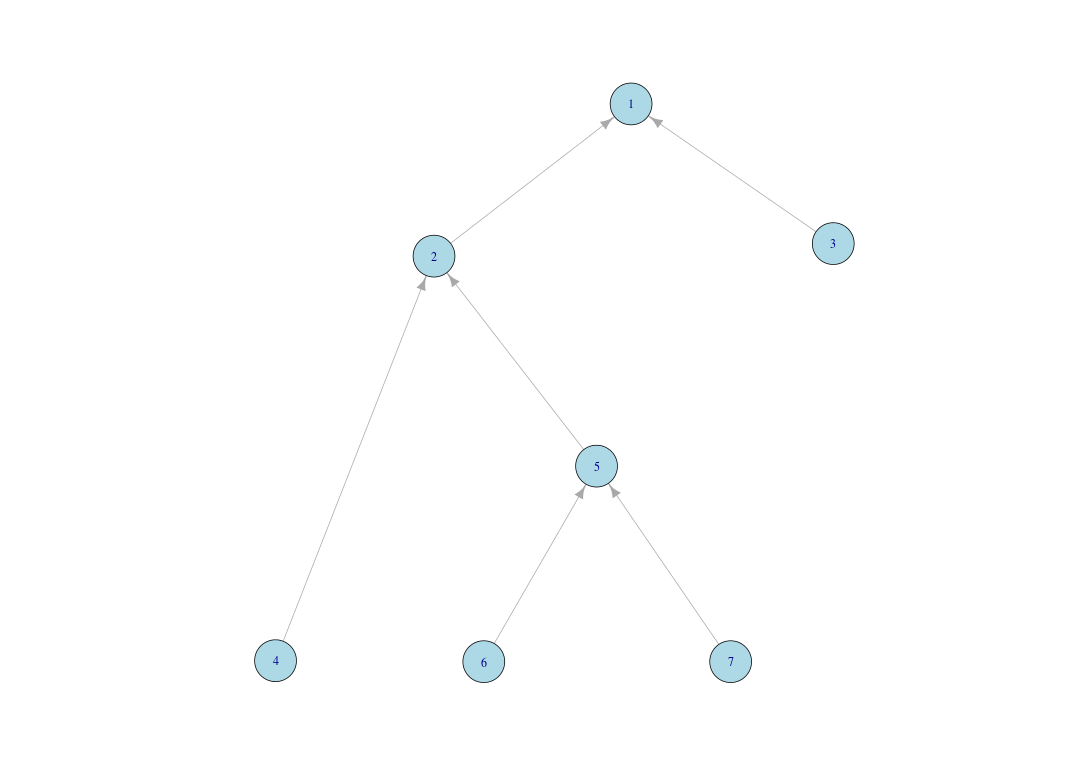
\includegraphics[width=0.45\textwidth]{/home/charles/Talks/Talk_2013Sep23/figures/network_original.eps} \\ 
 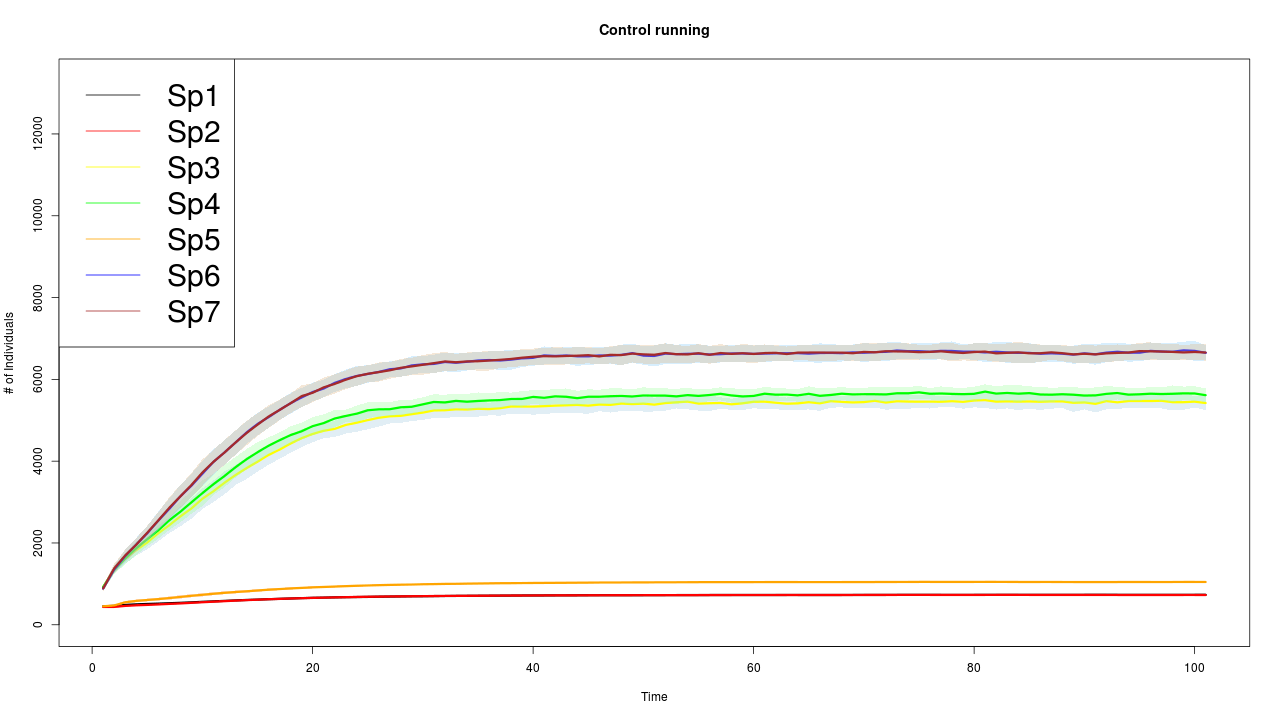
\includegraphics[width=0.55\textwidth]{/home/charles/Talks/Talk_2013Sep23/figures/AverageStdev_IndividualsInTime_Control.eps} 
\end{figure}
\end{frame}

\begin{frame}
\frametitle{Adding disturbance to the system}
\begin{figure}
 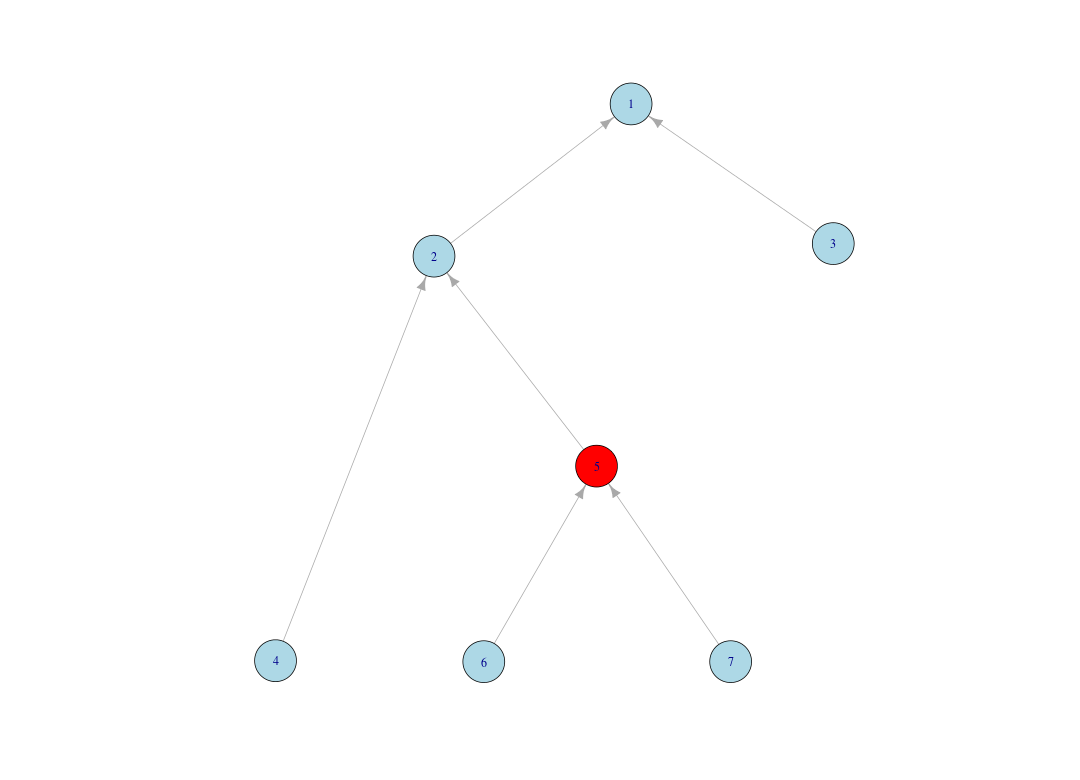
\includegraphics[width=0.45\textwidth]{/home/charles/Talks/Talk_2013Sep23/figures/network_decrease_5.eps} \\
 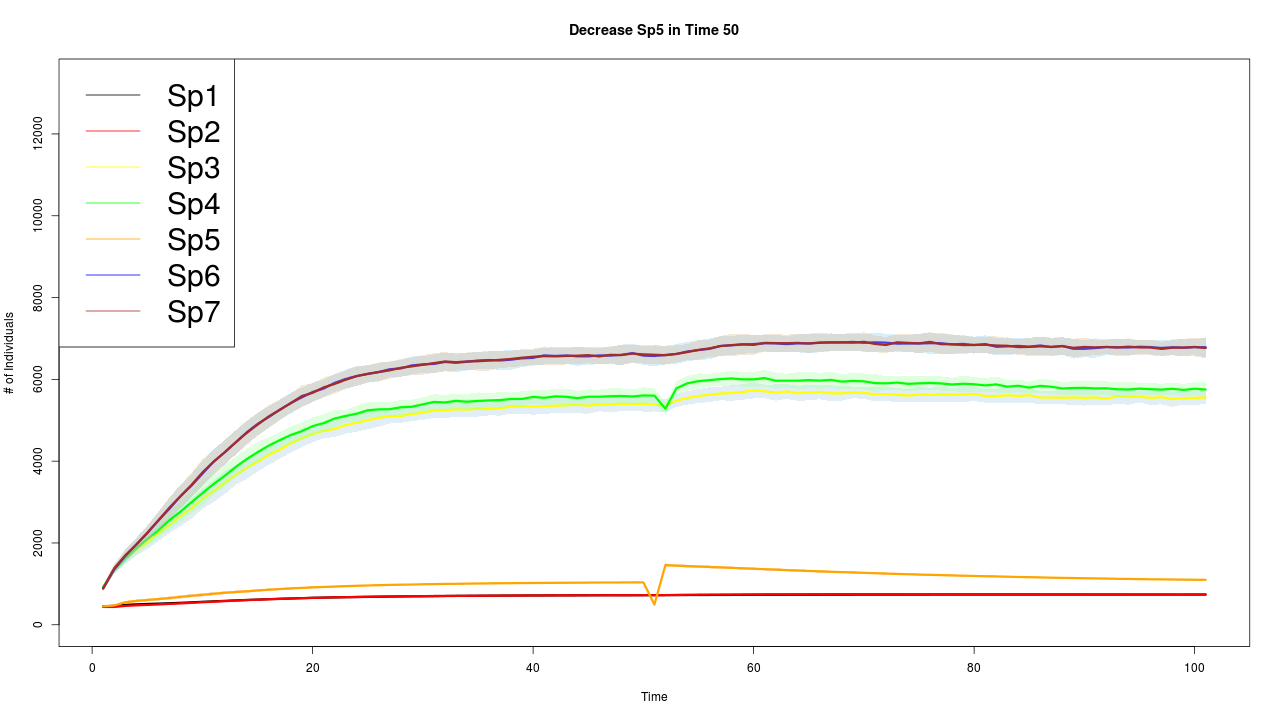
\includegraphics[width=0.55\textwidth]{/home/charles/Talks/Talk_2013Sep23/figures/AverageStdev_IndividualsInTime_Decrease_sp5_t50.eps}
\end{figure}
\end{frame}

\begin{frame}
\frametitle{Measuring the disturbance}
\begin{figure}
 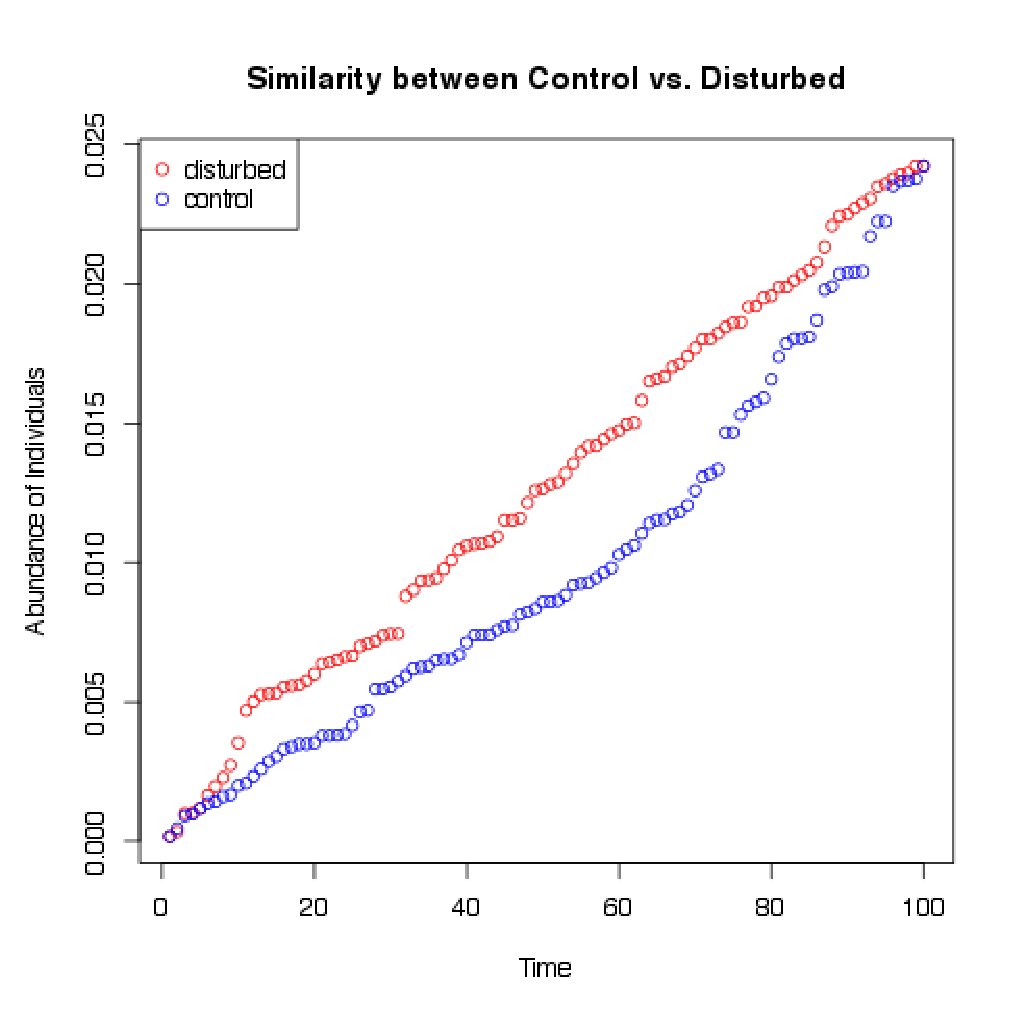
\includegraphics[width=0.5\textwidth]{/home/charles/Talks/Talk_2013Sep23/figures/perkins.eps} 
\end{figure}
\end{frame}

\begin{frame}
\frametitle{Case study: Resilience of an Antarctic Food Web}
\begin{figure}
 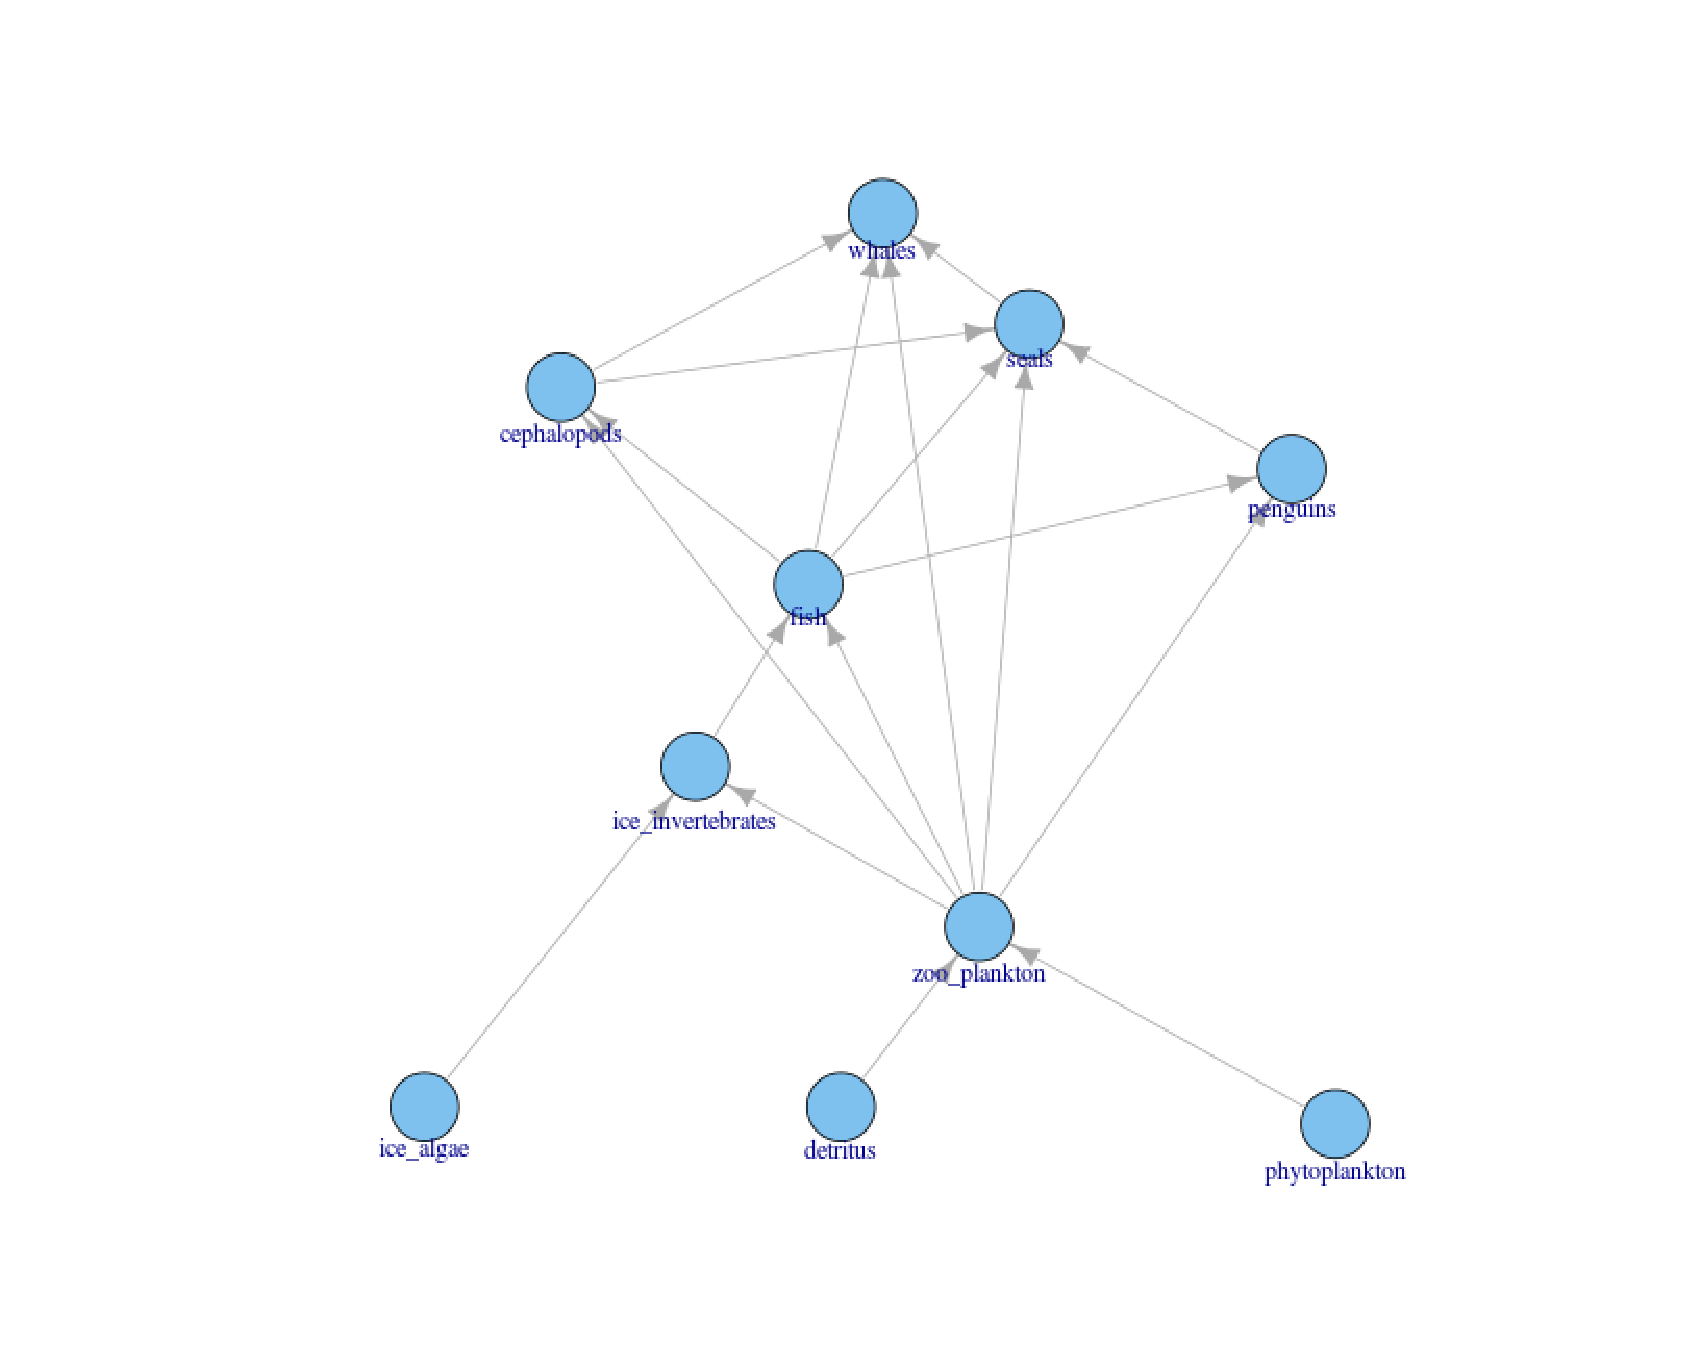
\includegraphics[width=0.55\textwidth]{/home/charles/Talks/Talk_2013Sep23/figures/antfigures/Antarctic_fweb.eps} 
 \includegraphics[width=0.45\textwidth]{/home/charles/Talks/Talk_2013Sep23/figures/antfigures/ant_control.eps}
\end{figure}
\end{frame}

\begin{frame}
\frametitle{Antarctic Food Web: decrease of abundance of species \emph{Zooplankton}}
\begin{figure}
 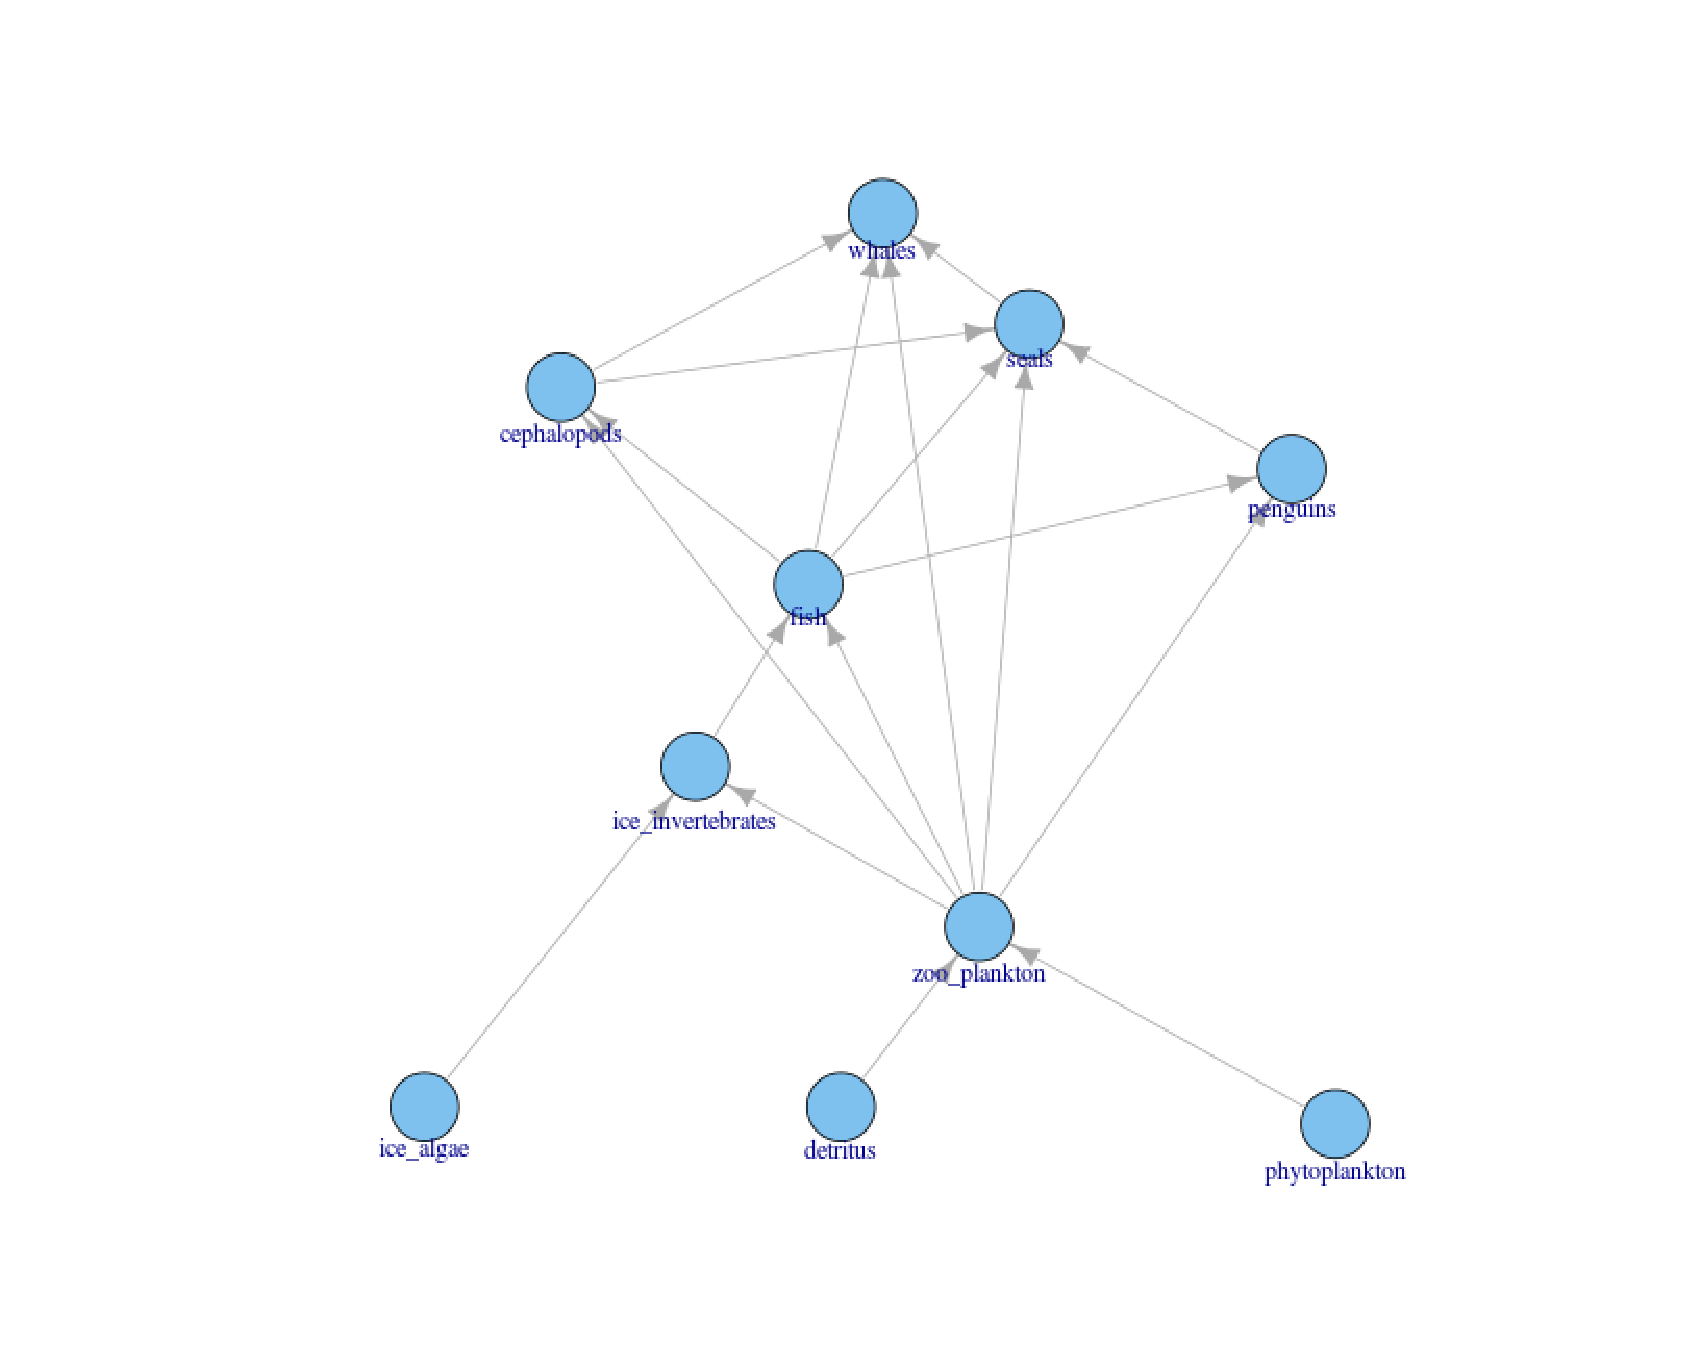
\includegraphics[width=0.55\textwidth]{/home/charles/Talks/Talk_2013Sep23/figures/antfigures/Antarctic_fweb.eps} 
 \includegraphics[width=0.45\textwidth]{/home/charles/Talks/Talk_2013Sep23/figures/antfigures/ant_dec05.eps} 
\end{figure}
\end{frame}

\begin{frame}
\frametitle{Effects of decrease in \emph{Zooplankton} in other species: \emph{Ice Algae}}
\begin{figure}
 \includegraphics[width=0.45\textwidth]{/home/charles/Talks/Talk_2013Sep23/figures/antfigures/ant_dec05.eps} 
 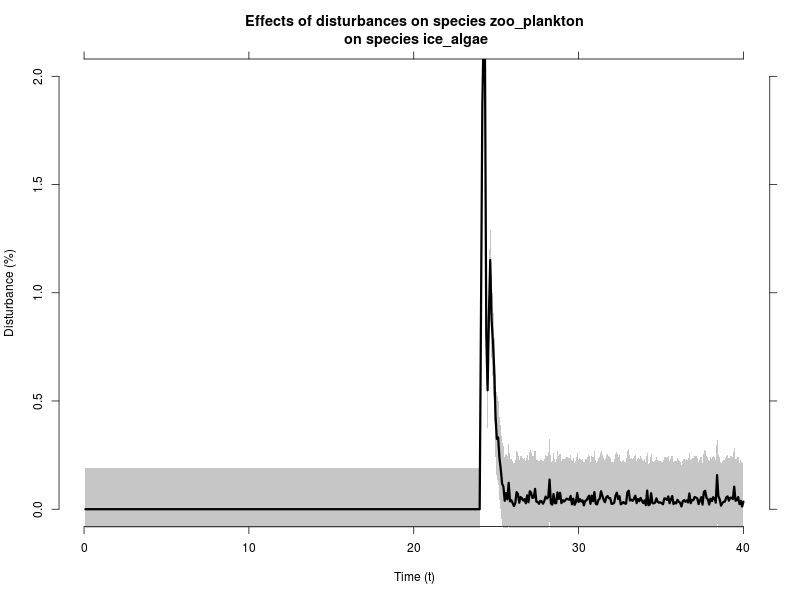
\includegraphics[width=0.55\textwidth]{/home/charles/Talks/Talk_2013Sep23/figures/antfigures/ant_stdevperkins_dec05_species_sp1}
\end{figure}
\end{frame}

\begin{frame}
\frametitle{Decrease in abundance of species: Effects among Trophic Levels}
\begin{figure}
 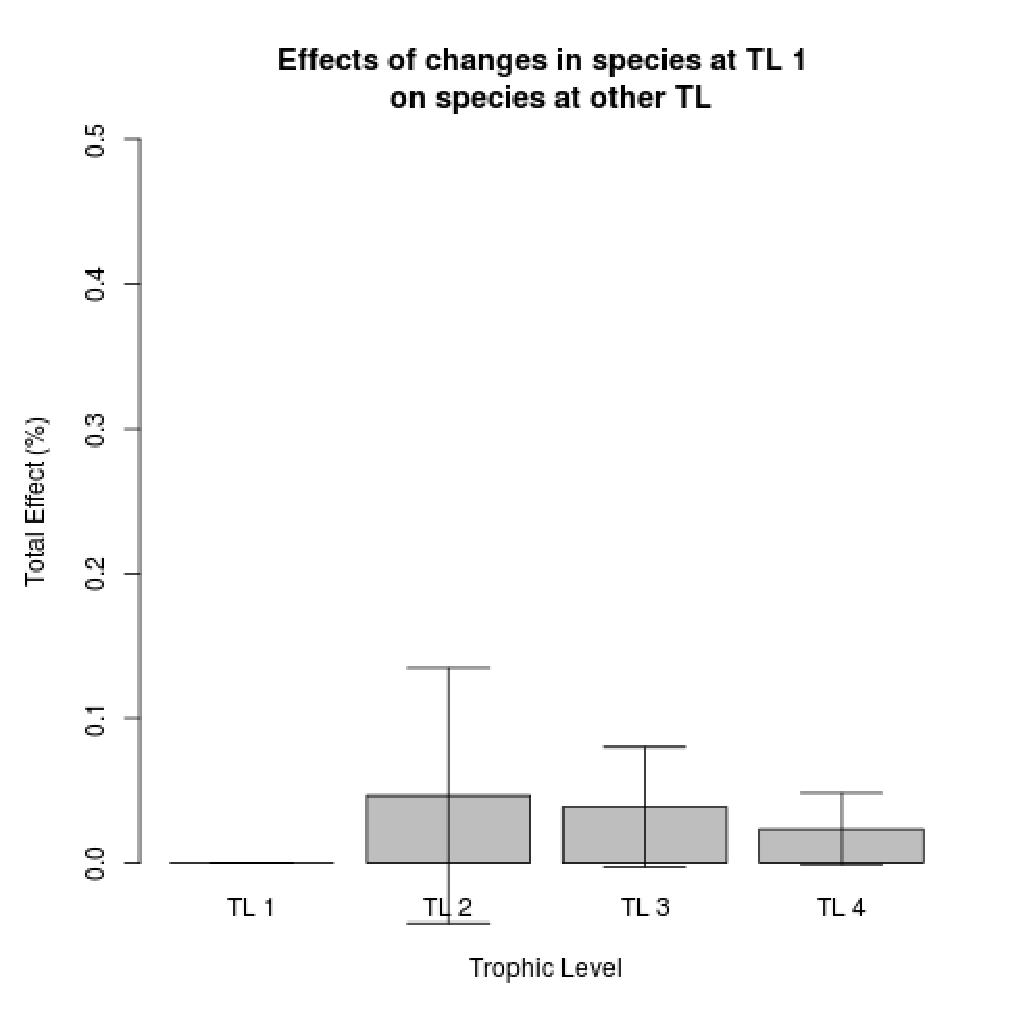
\includegraphics[width=0.45\textwidth]{/home/charles/Talks/Talk_2013Sep23/figures/antfigures/Effects_of_TL1} 
 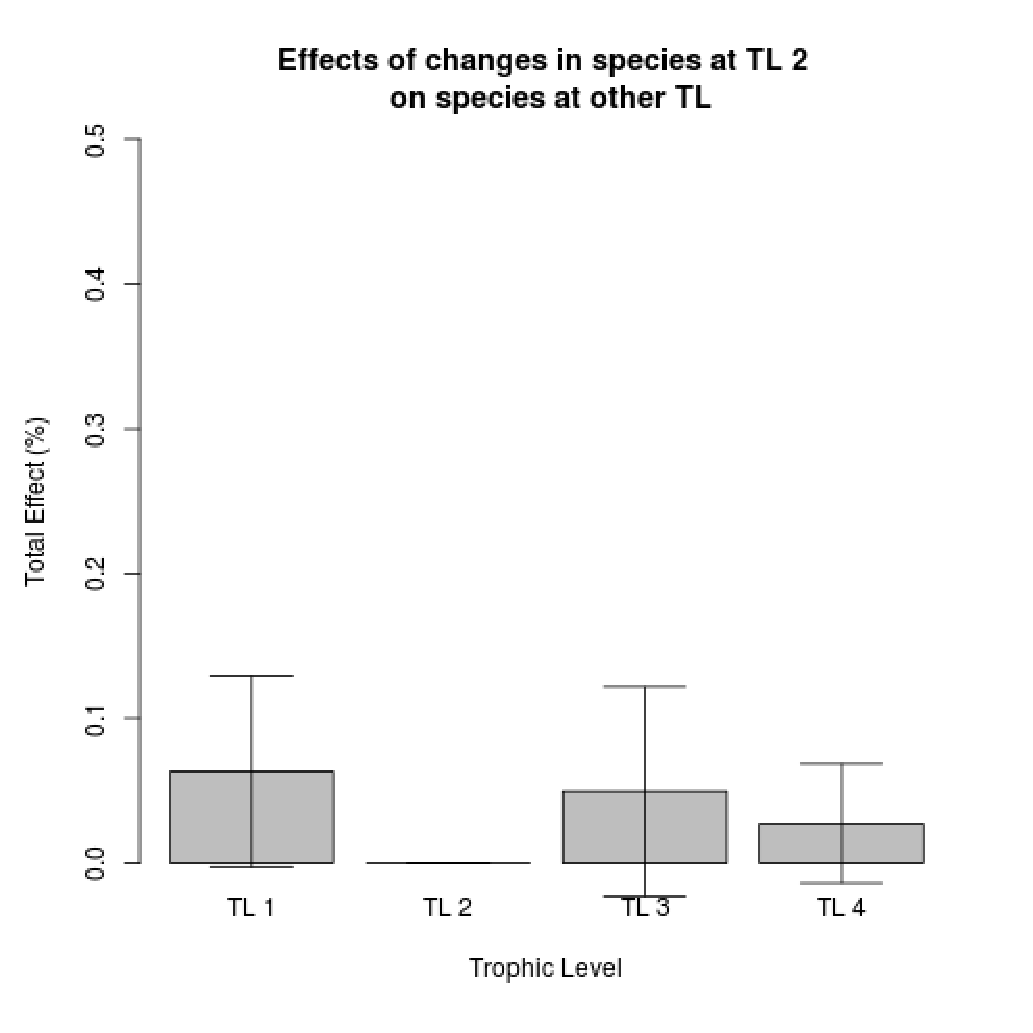
\includegraphics[width=0.45\textwidth]{/home/charles/Talks/Talk_2013Sep23/figures/antfigures/Effects_of_TL2} 
\end{figure}
\end{frame}

\begin{frame}
\frametitle{Decrease in abundance of species: Effects among Trophic Levels}
\begin{figure}
 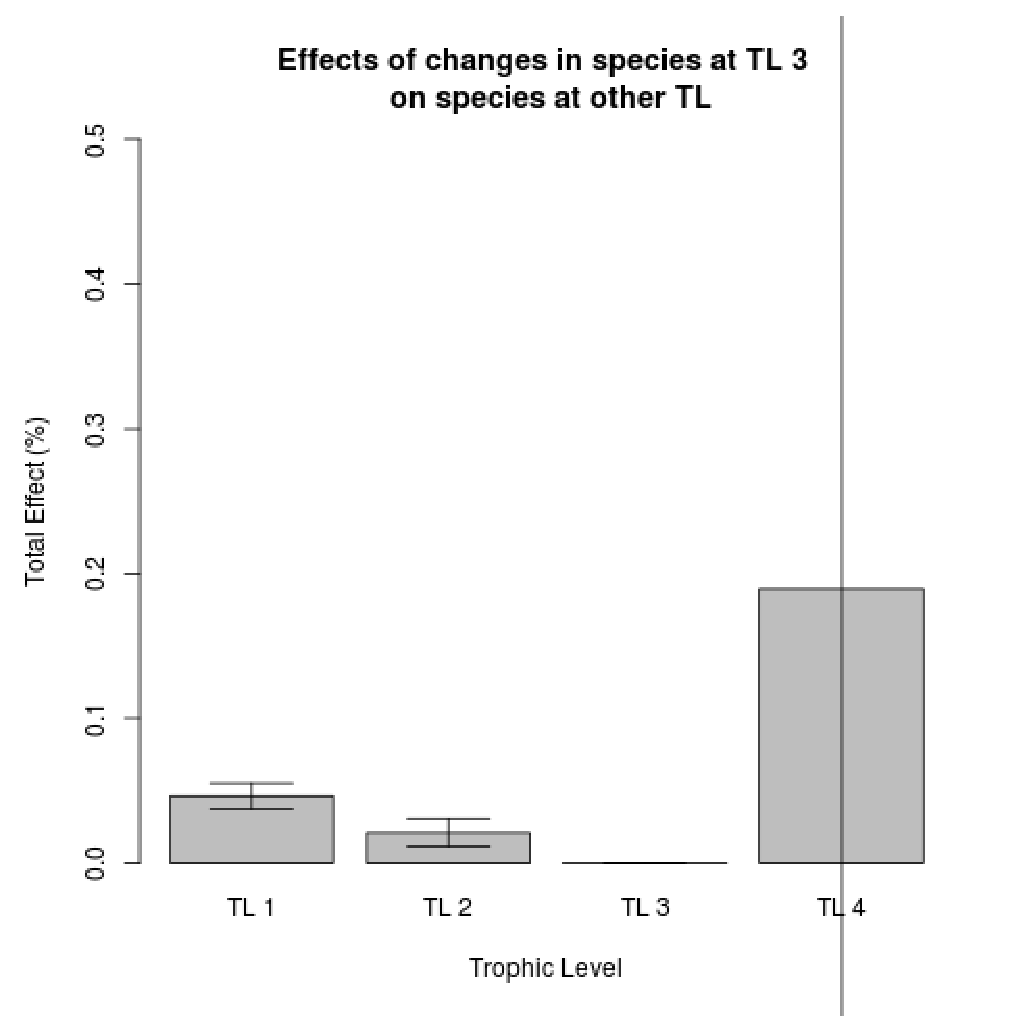
\includegraphics[width=0.45\textwidth]{/home/charles/Talks/Talk_2013Sep23/figures/antfigures/Effects_of_TL3} 
 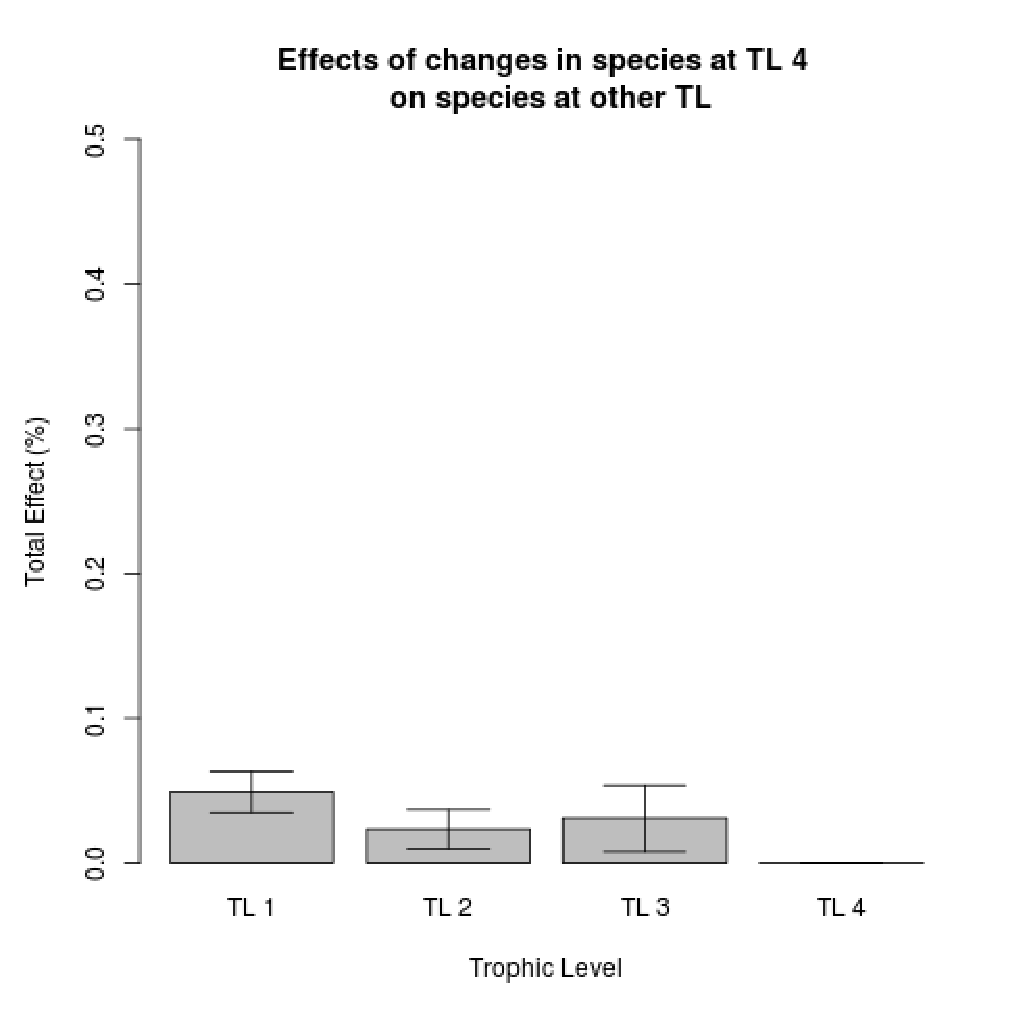
\includegraphics[width=0.45\textwidth]{/home/charles/Talks/Talk_2013Sep23/figures/antfigures/Effects_of_TL4} 
\end{figure}
\end{frame}

\begin{frame}
\frametitle{Studying Resilience of ecosystems}
\begin{block}{}
The model allow the addition of disturbances in the abundance of the species studied. By comparing the distribution of abundance of species in a \textbf{control run} and in different \textbf{disturbed run} we can infer characteristics about the resilience of the studied ecosystems. 
\end{block}
\end{frame}


%%%%%%%%%%% SPACE OF PARAMETERS

\subsection{Space of Parameters}
\begin{frame}
\frametitle{Space of Parameters: 30 species Food Web}
\begin{figure}
  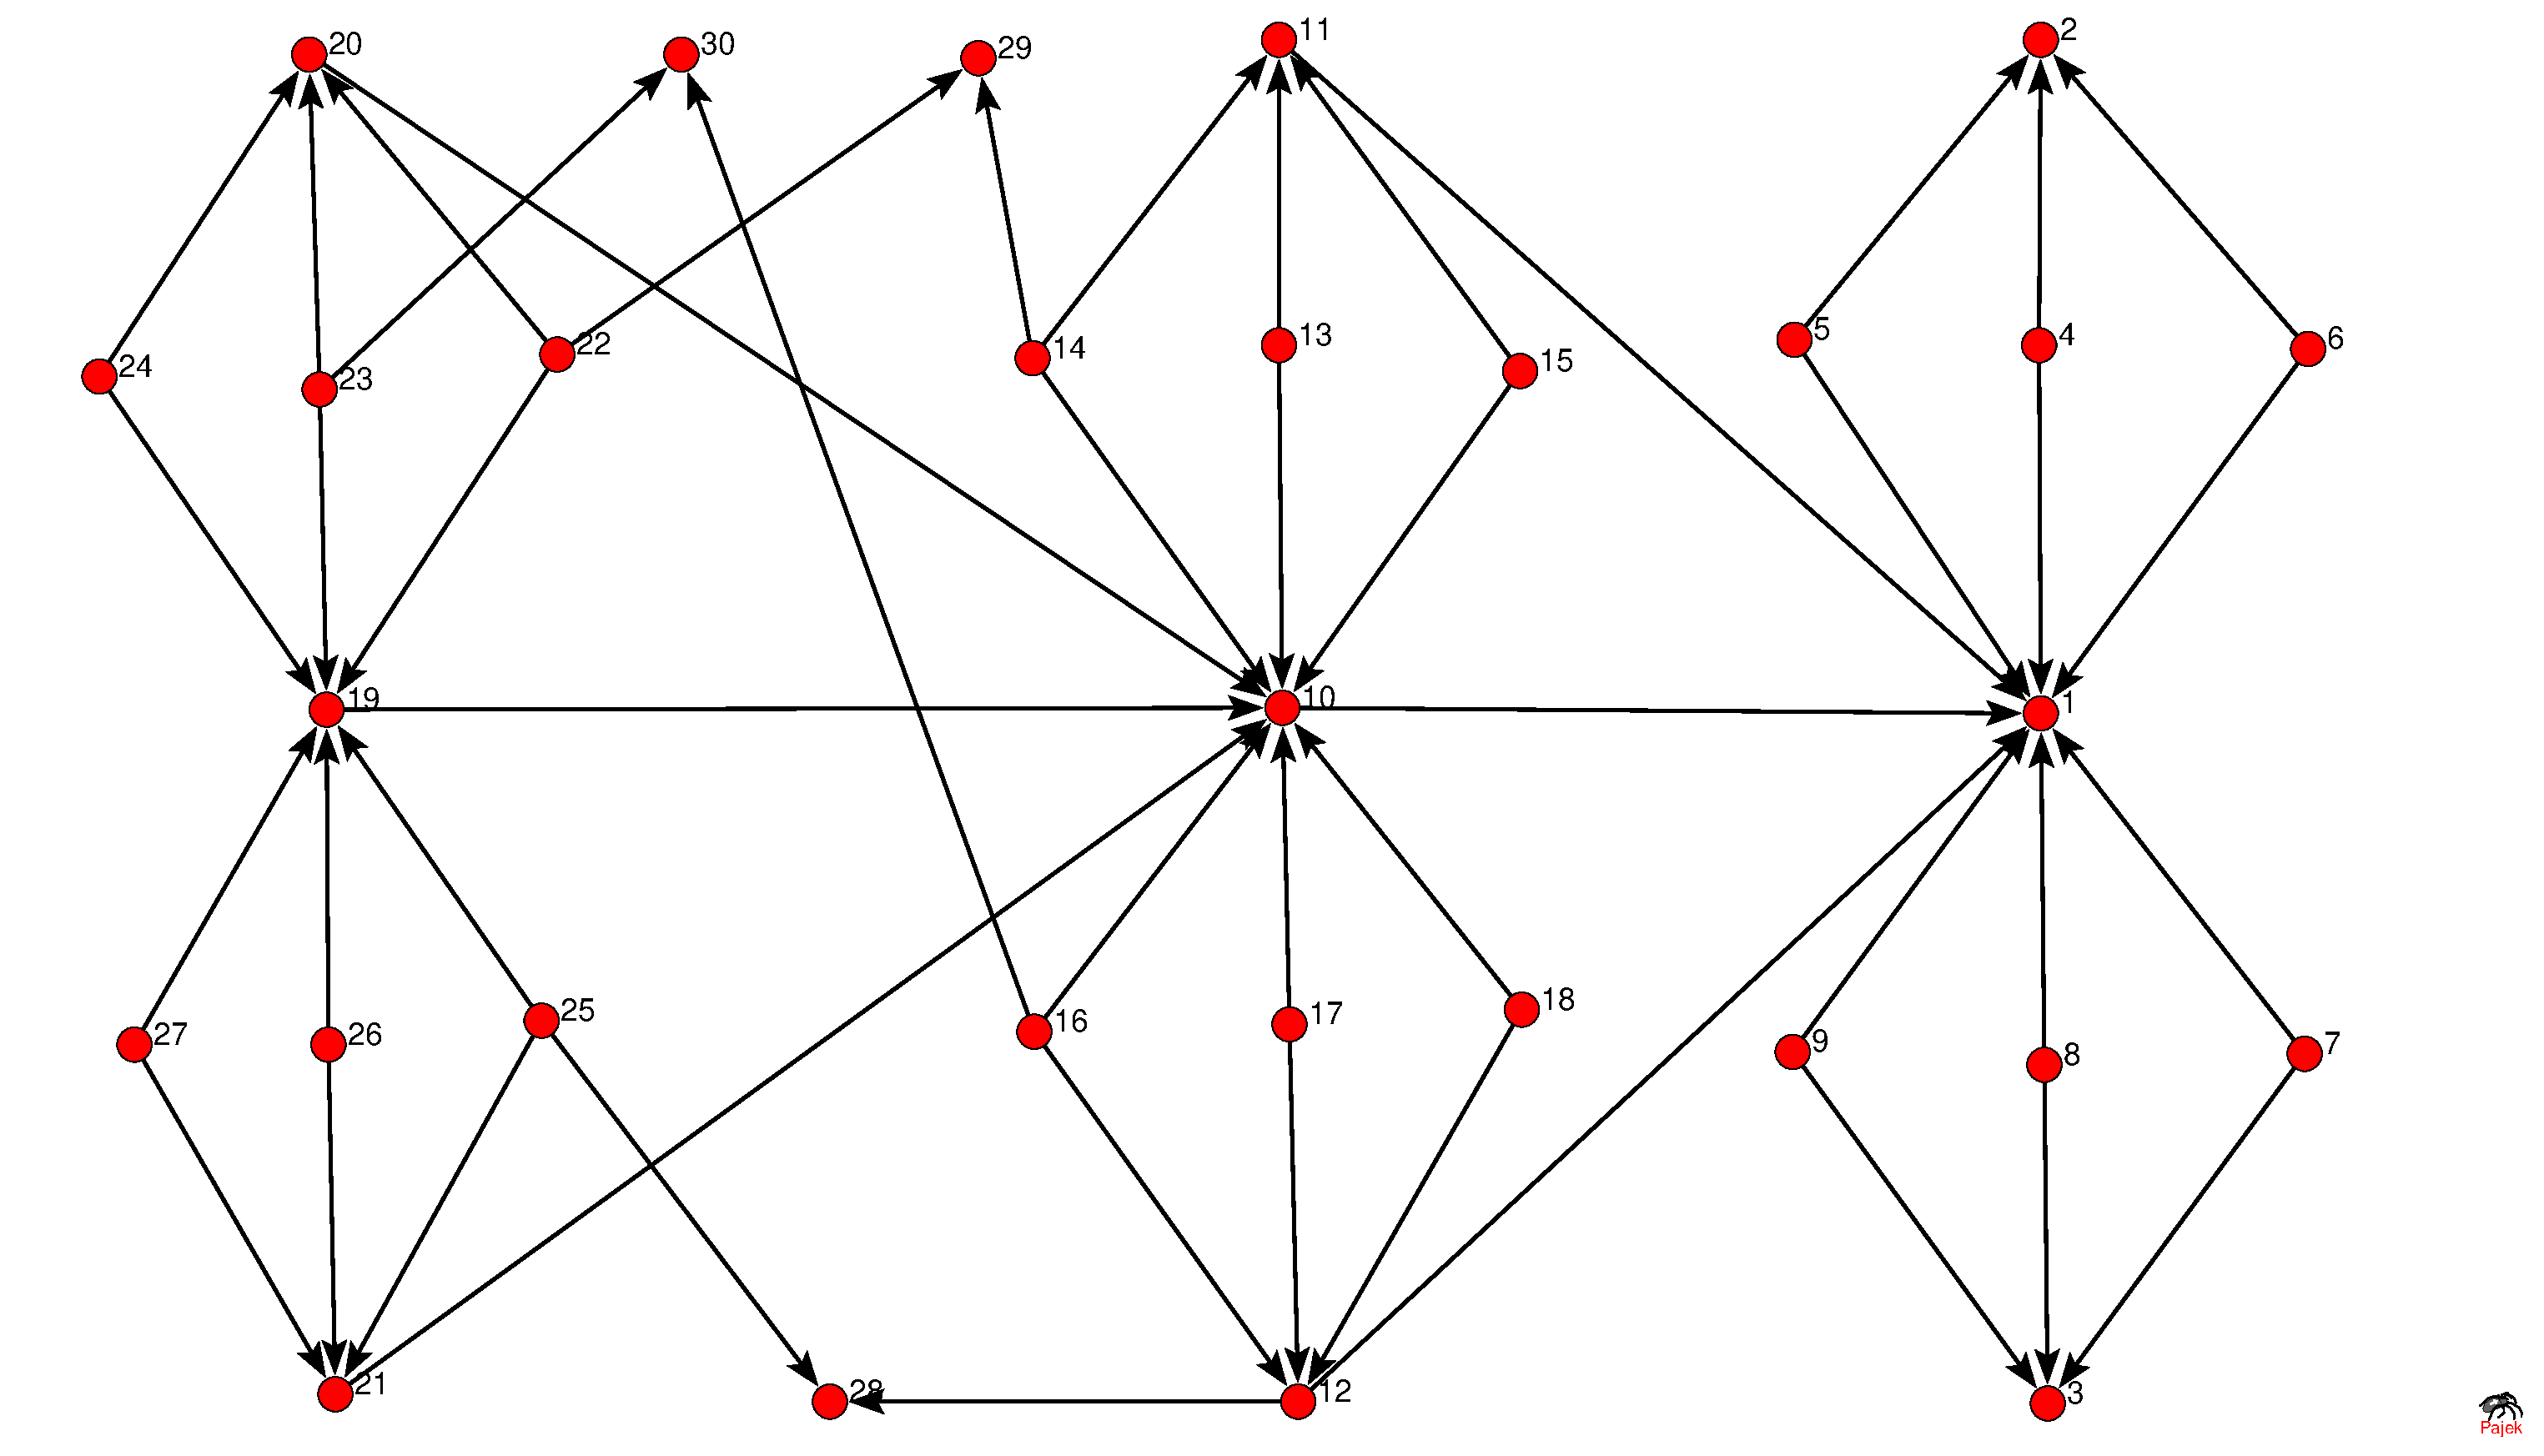
\includegraphics[width=1.0\textwidth]{/home/charles/Talks/Talk_2013Sep23/FoodWeb_30bloques9.eps}
\end{figure}
\end{frame}

\begin{frame}
\frametitle{30 species Food Web: Space of Bp}
\begin{columns}
  \begin{column}{0.5\textwidth}
   \begin{figure}
	\includegraphics[width=0.9\textwidth]{/home/charles/Talks/Talk_2013Sep23/TrophicLevels_30species}
   \end{figure}
  \end{column}

  \begin{column}{0.5\textwidth}
   \begin{figure}
	\includegraphics[width=1.0\textwidth]{/home/charles/Talks/Talk_2013Sep23/BP_at_s17_st71}
   \end{figure}
  \end{column}
\end{columns}
\end{frame}

\begin{frame}
\frametitle{Bp of a 30 Species Food Web}
\begin{block}{}
Aparently, in a \textbf{steady site}, the lower species' \textbf{trophic level} the higher species' \textbf{birth probability}. 
\end{block}
\end{frame}


%%%%%%%%%%%%% A L P H A 

\subsection{Metabolic Theory of Ecology}

\begin{frame}
\frametitle{Metabolic Rate: For a Food Web with 30 species}
\begin{figure}
  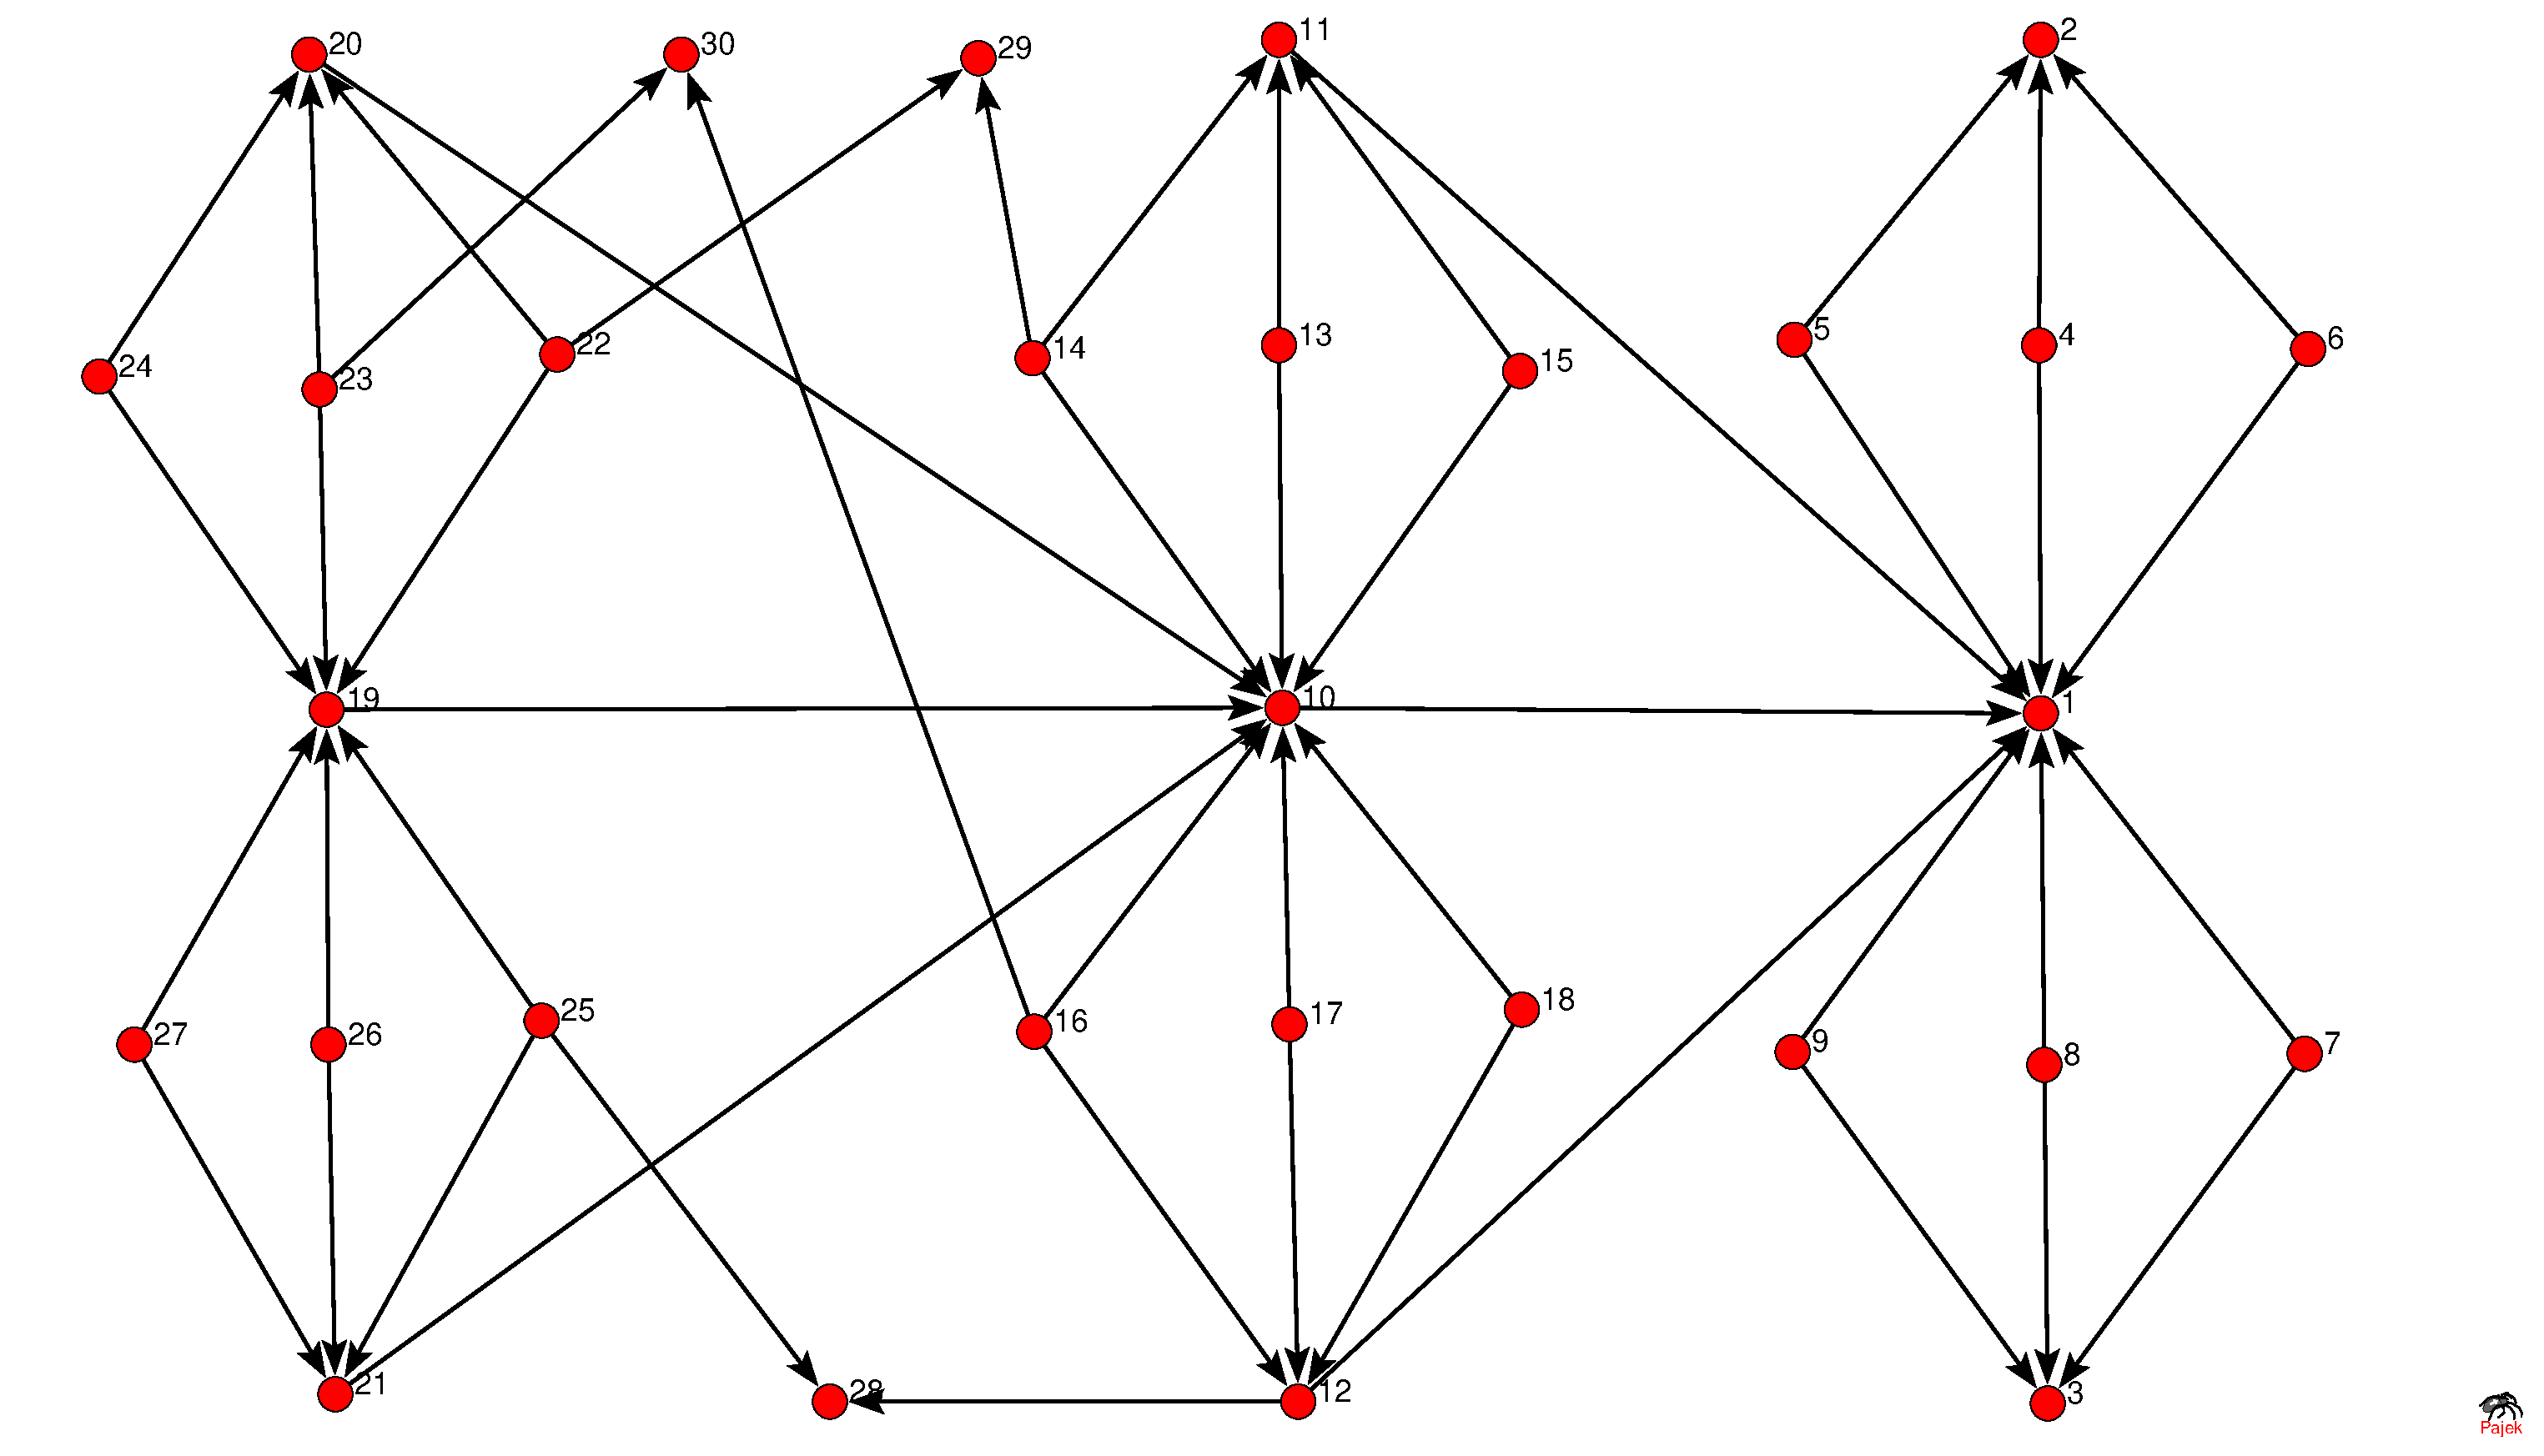
\includegraphics[width=0.75\textwidth]{/home/charles/Talks/Talk_2013Sep23/FoodWeb_30bloques9}
\end{figure}
\end{frame}

\begin{frame}
\frametitle{Metabolic Rate: $N \sim B^{\alpha}$ (for each site)}
\begin{figure}
  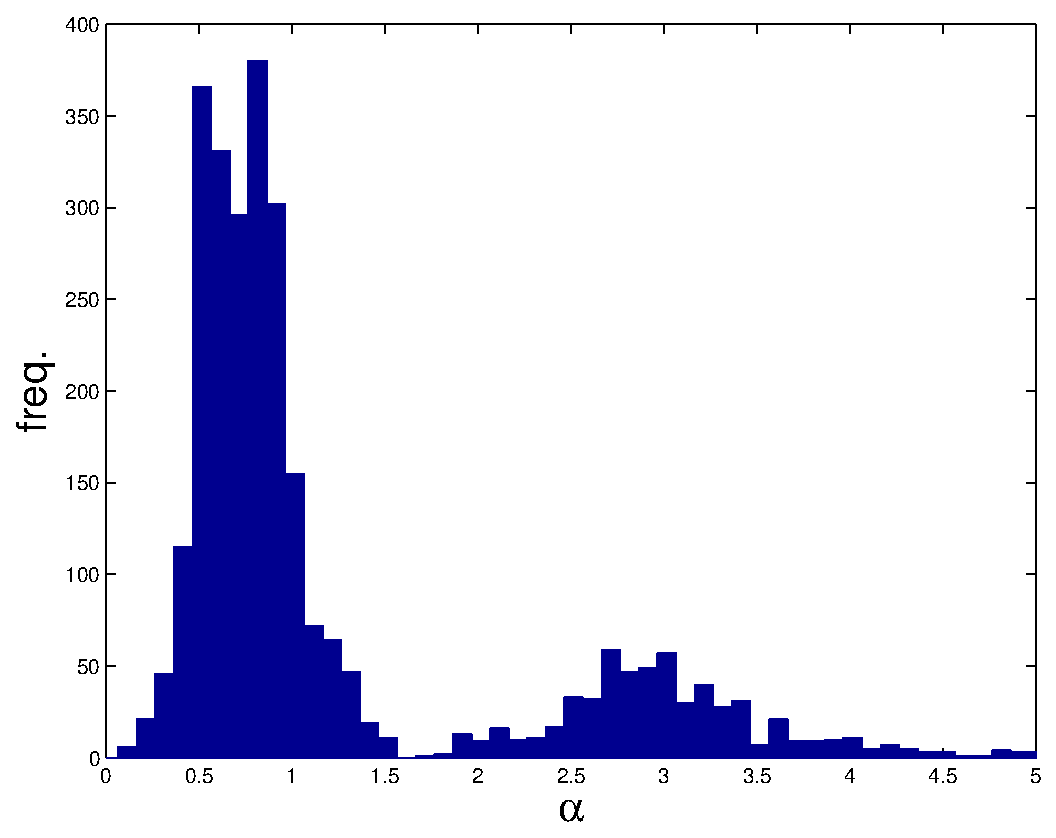
\includegraphics[width=0.75\textwidth]{/home/charles/Talks/Talk_2013Sep23/alpha_distr}
\end{figure}
\end{frame}

\begin{frame}
\frametitle{Metabolic Theory of Ecology}
\tikzstyle{na} = [baseline=-.5ex]

\begin{columns}
  \begin{column}{0.5\textwidth}
    \begin{itemize}
	\item \tikz[baseline]{\node[fill=red!20,ellipse,anchor=base] (t1) { $N$};} $\sim$ \tikz[baseline]{\node[fill=blue!20,ellipse,anchor=base] (t2) {$M^{ -\frac{3}{4} }$};} \tiny[1]
	\item \tikz[baseline]{\node[fill=yellow!20,ellipse,anchor=base] (t3) { $B$};} $\sim$ \tikz[baseline]{\node[fill=blue!20,ellipse,anchor=base] (t4) {$M^{ -\frac{1}{4} }$};} \tiny[2]
    \end{itemize}
  \end{column}

  \begin{column}{0.5\textwidth}
     \begin{itemize}[<2->]
	\item \tikz[baseline]{\node[fill=red!20,ellipse,anchor=base] (t5) { $N$};} $\sim$ \tikz[baseline]{\node[fill=yellow!20,ellipse,anchor=base] (t6) {$ B^{ 3 } $};}
     \end{itemize}
  \end{column}
\end{columns}
\begin{tikzpicture}[overlay]
        \path[->]<2-> (t1) edge [bend left] (t5);
        \path[->]<2-> (t3) edge [bend right] (t6);
\end{tikzpicture}
\vspace{1cm}
\begin{block}{}
{\footnotesize 1 - \textbf{Brown, J. H. , Gilloly, J. F. Allen, A. P., Savage V. M., and West G. B.} (2004). Toward a metabolic theory of ecology. \emph{Ecology}, 85:1171-1789.} \\
{\footnotesize 2 - \textbf{West, G. B., Brown, J. H.} (2005). The origin of allometric scaling laws in biology from genomes to ecosystems: towards a quantitative unifying theory of biological structure and organization. \emph{J Exp Biol}, 208:1575-1592.}
\end{block}
\end{frame}

\begin{frame}
\frametitle{Unestable Sites: $N \sim B^{1}$}
\begin{figure}
\includegraphics[width=0.25\textwidth]{/home/charles/Talks/Talk_2013Sep23/TS_s17_st13_Alpha_1_012.eps}
\includegraphics[width=0.25\textwidth]{/home/charles/Talks/Talk_2013Sep23/TS_s17_st24_Alpha_1_13.eps}
\end{figure}
\begin{figure}
\includegraphics[width=0.25\textwidth]{/home/charles/Talks/Talk_2013Sep23/TS_s17_st22_Alpha_0_96.eps}
\includegraphics[width=0.25\textwidth]{/home/charles/Talks/Talk_2013Sep23/TS_s17_st30_Alpha_0_58.eps}
\end{figure}
\end{frame}


\begin{frame}
\frametitle{Steady State Achieved Sites: $N \sim B^{3}$}
\begin{figure}
\includegraphics[width=0.25\textwidth]{/home/charles/Talks/Talk_2013Sep23/TS_s17_st29_Alpha_3_05}
\includegraphics[width=0.25\textwidth]{/home/charles/Talks/Talk_2013Sep23/TS_s17_st71_Alpha3_04}
\end{figure}
\begin{figure}
\includegraphics[width=0.25\textwidth]{/home/charles/Talks/Talk_2013Sep23/TS_s27_st2_Alpha2_99}
\includegraphics[width=0.25\textwidth]{/home/charles/Talks/Talk_2013Sep23/TS_s27_st33_Alpha2_85}
\end{figure}
\end{frame}

\begin{frame}
\frametitle{Methabolic Theory of Ecology}
\begin{block}{}
Aparently, there is a relation between a steady state achievement and the assessed $\alpha$ ($N \sim B^{\alpha}$) in the site. 
\end{block}
\end{frame}




%%%%%%%%%%%%%%%%%%%%%%%%%%%%%%%%%%%%%%%%%%%%%%%%%%%%%%%
\section{\scshape Conclusions}

\begin{frame}
\frametitle{Conclusions}
   \begin{figure}
	
\includegraphics[width=0.7\textwidth]{/home/charles/Talks/Talk_2013Sep23/conclusion.eps}
   \end{figure}
\end{frame}

\begin{frame}
\frametitle{Conclusions}

\begin{block}{}
Expressing the parameters that govern the dynamics as functions of densities, we introduce correlations between Bp, Dp, NDp. As a result of that, the system \textbf{self-organizes towards steady state}, independently of the initial number of individuals. 
\end{block}
\pause

\begin{block}{}
The model allow the comparison of dynamics of the simulated systems under different disturbed situation: (e.g.: loss of habitat; changes in niche of species; loss of connectivity between sites; invasive species; extinction of species; etc). 
\end{block}
\pause

\begin{block}{}
Aparently, in a \textbf{steady site}, the lower species' \textbf{trophic level} the higher species' \textbf{birth probability}.
\end{block}
\pause

\begin{block}{}
Aparently, there is a relation between a steady state achievement and the assessed $\alpha$ ($N \sim B^{\alpha}$) within each site. 
\end{block}
\pause

\end{frame}

\begin{frame}

\frametitle{Conclusions}

\begin{block}{}
The model is general enough to allow the inclusion of biotic and abiotic iterations. 
\end{block}
\pause

\begin{block}{}
The model can be nested to niche models, and then provide a \emph{Niche Model with Biotic Iteractions}.
\end{block}
\pause

%\begin{block}{}
%The model allow the inclusion of global changes signs, by changing parameters $w_{i,j}$ and $\Delta^{i,j} f_{\eta}$. 
%\end{block}
%\pause

\end{frame}

\begin{frame}{Thannk you for your attention!}
\end{frame}


%%%%%%%%%%%%%%%%%%%%%%%%%%%%%%%%%%%%%%%%%%%%%%%%%%%%%%%
%%%%%%%%%%%%%%%%%%%%%%%%%%%%%%%%%%%%%%%%%%%%%%%%%%%%%%
%%%%%%%%%%%%%%%%%%%%%%%%%%%%%%%%%%%%%%%%%%%%%%%%%%%%%%%
%%%%%%%%%%%%%%%%%%%%%%%%%%%%%%%%%%%%%%%%%%%%%%%%%%%%%%
%%%%%%%%%%%%%%%%%%%%%%%%%%%%%%%%%%%%%%%%%%%%%%%%%%%%%%

\end{document}
